%%%%%%%%%%%%%%%%%%%%%%%%%%%%%%%%%%%%%%%%%%%%%%%%%%%
%% LaTeX book template                           %%
%% Author:  Amber Jain (http://amberj.devio.us/) %%
%% License: ISC license                          %%
%%%%%%%%%%%%%%%%%%%%%%%%%%%%%%%%%%%%%%%%%%%%%%%%%%%

\documentclass[a4paper,11pt]{book}
\usepackage{lipsum}
\usepackage[Lenny]{fncychap}
\ChNameUpperCase
\ChTitleUpperCase
\ChNumVar{\fontsize{40}{42}\usefont{OT1}{ptm}{m}{n}\selectfont}
% \ChTitleVar{\Large\sc}

\usepackage[T1]{fontenc}
\usepackage[utf8]{inputenc}
\usepackage{lmodern}
\usepackage{subcaption}
\usepackage{hyperref}
\usepackage{xcolor}
\usepackage{amsmath}
\usepackage{wrapfig}    % inline figures
\usepackage{enumitem}
\usepackage{comment}
\usepackage{lipsum}
\usepackage{graphicx} % Use for Images
\usepackage{here}     % Forced Figure Placement
\usepackage{pslatex}	% Use PostScript Fonts
\usepackage{fancyhdr} % Use headers
\usepackage{float}
%%%%%%%%%%%%%%%%%%%%%%%%%%%%%%%%%%%%%%%%%%%%%%%%%%%%%%%%%
% Source: http://en.wikibooks.org/wiki/LaTeX/Hyperlinks %
%%%%%%%%%%%%%%%%%%%%%%%%%%%%%%%%%%%%%%%%%%%%%%%%%%%%%%%%%
\usepackage{hyperref}
\usepackage{graphicx}
% \usepackage{algopseudocode}
\usepackage{algorithm}
\usepackage{algorithmic}
\usepackage{amssymb}
\usepackage[english]{babel}
% \usepackage{biblatex}

\usepackage[
	top    = 1cm,
	bottom = 1.80cm,
	left   = 2.00cm,
	right  = 2.00cm,
	includeheadfoot]{geometry} % Use similar margins to the Word Template
\setlength{\parindent}{0pt}



%%%%%%%%%%%%%%%%%%%%%%%%%%%%%%%%%%%%%%%%%%%%%%%%%%%%%%%%%
% Source: http://en.wikibooks.org/wiki/LaTeX/Hyperlinks %
%%%%%%%%%%%%%%%%%%%%%%%%%%%%%%%%%%%%%%%%%%%%%%%%%%%%%%%%%
\usepackage{hyperref}
\usepackage{graphicx}
\usepackage[english]{babel}
% \usepackage{biblatex}
% \usepackage[refsection=chapter]{biblatex}
% \usepackage{biblatex}
\usepackage[
backend=biber,
sorting=none
]{biblatex}
\addbibresource{My Library.bib}
% \bibliographystyle{unsrt}
%%%%%%%%%%%%%%%%%%%%%%%%%%%%%%%%%%%%%%%%%%%%%%%%%%%%%%%%%%%%%%%%%%%%%%%%%%%%%%%%
% 'dedication' environment: To add a dedication paragraph at the start of book %
% Source: http://www.tug.org/pipermail/texhax/2010-June/015184.html            %
%%%%%%%%%%%%%%%%%%%%%%%%%%%%%%%%%%%%%%%%%%%%%%%%%%%%%%%%%%%%%%%%%%%%%%%%%%%%%%%%
\let\cleardoublepage\clearpage
\newenvironment{dedication}
{
   \cleardoublepage
   \thispagestyle{empty}
   \vspace*{\stretch{1}}
   \hfill\begin{minipage}[t]{0.66\textwidth}
   \raggedright
}
{
   \end{minipage}
   \vspace*{\stretch{3}}
  %  \clearpage
}

%%%%%%%%%%%%%%%%%%%%%%%%%%%%%%%%%%%%%%%%%%%%%%%%
% Chapter quote at the start of chapter        %
% Source: http://tex.stackexchange.com/a/53380 %
%%%%%%%%%%%%%%%%%%%%%%%%%%%%%%%%%%%%%%%%%%%%%%%%
% \makeatletter
% \renewcommand{\@chapapp}{}% Not necessary...
% \newenvironment{chapquote}[2][2em]
%   {\setlength{\@tempdima}{#1}%
%    \def\chapquote@author{#2}%
%    \parshape 1 \@tempdima \dimexpr\textwidth-2\@tempdima\relax%
%    \itshape}
%   {\par\normalfont\hfill--\ \chapquote@author\hspace*{\@tempdima}\par\bigskip}
% \makeatother


% Define the page styles
\fancypagestyle{titlepage}{
	\fancyhf{}
	\fancyhead[C]{
\includegraphics[width=\textwidth]{images/banner.png}}
	\renewcommand{\headrulewidth}{1pt}
}

%\fancypagestyle{body}{
%	\fancyhf{}
%  \fancyhead[C]{
\includegraphics{images/banner.png}}
%}

\fancypagestyle{body}{
    \fancyhf{}
    \fancyhead[C]{
\includegraphics[width=.8\textwidth]{images/banner.png}}
    \setlength{\headsep}{8pt}
    \addtolength{\topmargin}{-45.11401pt}
    \setlength{\headheight}{77.11401pt}
    \fancyhead[LE,RO]{\thepage}
    % \renewcommand{\headrulewidth}{.4pt}
    % \renewcommand\plainheadrulewidth{.4pt}
    % \fancyhead[RE,LO]{Chapter \leftmark}
    
}
\patchcmd{\chapter}{\thispagestyle{plain}}{\thispagestyle{fancy}}{}{}

\fancypagestyle{contents}{
    % \fancyhf{}
    % \fancyhead[LE,RO]{\thepage}
    % \fancyhead[RE,LO]{\leftmark}
    \fancyhf{}
    \fancyhead[C]{
\includegraphics[width=.8\textwidth]{images/banner.png}}
    \setlength{\headsep}{1pt}
    \addtolength{\topmargin}{-45.11401pt}
    \setlength{\headheight}{77.11401pt}
    \fancyhead[LE,RO]{\thepage}
    \renewcommand{\headrulewidth}{.8pt}


}

\fancypagestyle{appendix}{
    % \fancyhf{}
    % \fancyhead[LE,RO]{\thepage}
    % \fancyhead[RE,LO]{APPENDICES}
    \fancyhf{}
    \fancyhead[C]{
\includegraphics[width=.8\textwidth]{images/banner.png}}
    \setlength{\headsep}{1pt}
    \addtolength{\topmargin}{-45.11401pt}
    \setlength{\headheight}{77.11401pt}
    \fancyhead[LE,RO]{\thepage}
    \renewcommand{\headrulewidth}{.8pt}


}

\fancypagestyle{acknowledgements}{
    \fancyhf{}
    \fancyhead[LE,RO]{\thepage}
}


\renewcommand{\headrulewidth}{1.5pt}
\renewcommand{\arraystretch}{1.2}
\usepackage{tabularx}


%%%%%%%%%%%%%%%%%%%%%%%%%%%%%%%%%%%%%%%%%%%%%%%%%%%
% First page of book which contains 'stuff' like: %
%  - Book title, subtitle                         %
%  - Book author name                             %
%%%%%%%%%%%%%%%%%%%%%%%%%%%%%%%%%%%%%%%%%%%%%%%%%%%

% % Book's title and subtitle
% \title{\Huge \textbf{Sample Book Title}  \footnote{This is a footnote.} \\ \huge Sample book subtitle \footnote{This is yet another footnote.}}
% % Author
% \author{\textsc{First-name Last-name}\thanks{\url{www.example.com}}}
\title{
    % \vspace{1cm}
    \centering
\includegraphics[width=\textwidth]{images/banner.png}
    \vspace{5mm}
        {\bf
        {\Huge Proxy Attention : Comparing and Combining Augmentation with Attention\\
        % \vspace{2mm}Som\\
        }
        }
        \vspace{4mm}Graduation Project\\(Computational Intelligence and Robotics)\\
        \vspace{4mm}Subhaditya Mukherjee (s4747925)\\ \today \\
        \vspace{5cm}{\LARGE Internal Supervisor: S.H. Mohades Kasaei, PhD\\ Second Internal Supervisor: Matias Valdenegro, PhD\\ (Artificial Intelligence, University of Groningen)}\\
        {\bf {Artificial Intelligence\\University of Groningen, The Netherlands}}
}
\date{}

\pagestyle{body}% Set page style to plain
\begin{document}
% \thispagestyle{body}
\maketitle

% \setlength{\headheight}{32pt}

% \thispagestyle{body}
\tableofcontents

% \thispagestyle{body}
\listoffigures

% \thispagestyle{body}
\listoftables


\chapter*{Key}

\begin{enumerate}
    \item $\odot$ denotes element-wise multiplication
\end{enumerate}

% \thispagestyle{acknowledgements}    % remove this if you want `CONTENTS' to appear in the header of the first Contents page
% \pagestyle{contents}

%\setlength{\headheight}{32pt}

\tableofcontents
\addtocontents{toc}{~\hfill\textbf{Page}\par}

% incase the contents spill onto another page use this for help: https://tex.stackexchange.com/questions/8296/add-page-above-page-numbers-in-table-of-contents

% \include{chapters/acknowledgements}
% \thispagestyle{body}
\section{Introduction}
Over the past decade or so, Computer Vision (CV) has taken over the world. Almost every domain, ranging from medicine to robotics has been affected in some way or the other because of it. At the heart of all of these improvements, reside Neural Network architectures. There are thousands of architectures, each made to serve a different purpose, some vastly better than the other. But for each of them, there exists tradeoffs. Accuracy, Memory, Time to train, Cost to run etc. Scaling up these models requires a massive amount of energy, with some consuming upwards of 27,648 kilowatt hours of electricity just to train. This is around the same amount that three households use in a whole year. \href{https://www.techtarget.com/searchenterpriseai/feature/Energy-consumption-of-AI-poses-environmental-problems}{source}. And this is just one model.\\
In order to get any kind of prediction from them, these networks need to be fed large quantities of data. This training consumes a vast amount of resources that becomes increasingly harder to provide in niche problems where only a small amount of data is available. Models that outperform existing benchmarks such as the Swin Transformer \cite{liu_swin_2022} require an abysmal amount of data and energy. This makes it extremely hard for smaller companies, research labs and individuals to use this technology.\\
The second major flaw of these systems is due to the extremely complex, high dimensional manifolds they try to model. Because of such high dimensionality, it becomes next to impossible to predict exactly why a network made the decision it did. This becomes extremely important in situations like performing medical diagnoses. Not knowing why a network said what it did, makes it very hard to trust. The rise of Explainable AI (XAI) attempts to solve this issue.\\
In order to tackle the lack of data, many methods such as transforming the present data in multiple ways to increase the available data points aka data augmentation have been created. Methods like transfer learning enable using pre-trained networks to "fine-tune" on a specific dataset. In the traditional sense, the fields of XAI and data augmentation are not related. So far, the outputs of XAI algorithms have just been used as an explainibility measure, not for training.
Therefore, combining these concepts, we arrive at a novel Augmentation technique that uses Saliency maps as an input during training to emulate Attention \cite{vaswani_attention_2017} mechanisms. We call this "Proxy Attention".\\
The objective of this thesis is to design a novel informed augmentation method that would not only reduce the requirement of data, but will also be more memory and time efficient during training as compared to current algorithms in turn building on the advances of XAI to improve training performance.
% \thispagestyle{body}
\chapter{Background}
\section{Interpretability}
\begin{itemize}
\item Need for Interpretability
\end{itemize}
\section{Gradient Based Explanations}
\begin{itemize}
\item Taxonomy
\end{itemize}
\section{Augmentation}
\begin{itemize}
\item Taxonomy
\end{itemize}
\section{Datasets}
CIFAR 100

IIT pets

stanford dogs

imagenette

ASL
% \thispagestyle{body}
\chapter{State of the Art}
\section{Gradient Based Explanations}
% Deconvnet
One of the earlier approaches to Saliency maps for CNNs was proposed by Zeiler et al. \cite{zeilerVisualizingUnderstandingConvolutional2013} termed DeconvNet. DeconvNet works by inverting the network's operations in the forward pass. After attaching the DeconvNet layers to the network, propagating through these layers represents features that the original CNN possessed. The relevant reconstruction can be obtained for a single class by setting all the activations other than the one corresponding to the class to zero. The resulting image is then used to generate the saliency map. A Deconv layer replaces the Conv layer, and the ReLU operation has negative values clamped. While the pooling operation is not strictly invertible, the authors use switch variables that store the maximum value position for each pooling operation. While the DeconvNet works to a certain extent, the results are less accurate than the ones obtained by other methods and are also biased towards the representations of the first layer.

% Deep Inside Conv Nets
Building on the DeconvNet, Simonyan et al. \cite{simonyanDeepConvolutionalNetworks2014} extrapolate the idea of class visualization to create one of the first approaches to Saliency maps. Their approach, also called Vanilla Gradient, ranks the pixels of an image $I_{0}$ by how important they are in the prediction of the Saliency score $S_{c}(I) \approx w^{T}I + b$. In this equation, $w$ and $b$ are the network weights and biases obtained by back-propagating wrt the image itself. The objective to be minimized thus is $arg \underset{I}max S_{c}(I) - \lambda||I||^{2}_{2}$ where $\lambda$ is used as a regularization parameter. Using these equations, a saliency map $A \in \mathbb{R}^{m \times n}$ ($m \times n$ stands for $height \times width$) can be computed. To find the map, we find the derivative of $w$, rearrange the elements and then process them according to the number of input channels. If the number of channels is greater than one, the maximum value over the channel is considered $A_{i,j}= \underset{ch}max |w_{h_{(i,j, ch)}}|$. Where $ch$ is the colour channel of the pixel $(i,j)$, $h(i,j, ch)$ is the index of the $w$ corresponding to that pixel. The Vanilla Gradient method produces an approximate saliency map but has much noise. This leads to issues for more complex images. The methods proposed in the following papers have addressed many of the issues with Vanilla Gradients and DeconvNets \cite{zeilerVisualizingUnderstandingConvolutional2013}.

% Scorecam
In another paper, the authors propose a score-weighted approach - ScoreCAM to create saliency maps \cite{wangScoreCAMScoreWeightedVisual2020}. Like many other methods, the images are first passed through the network, and the corresponding activations are obtained from the final convolutional layer. These activation maps are upsampled and normalized to $[0,1]$. The highlighted activation map portions are then passed through a CNN with a SoftMax layer to obtain the score for each of the current classes. These scores are used to find the activation maps' relative importance. Finally, the sum of all these maps is computed using a linear combination with the corresponding target score and then passed through a ReLU operation. These operations can be mathematically represented as $L^{c}_{ScoreCAM} = ReLU(\underset{k}\Sigma w_{k}^{c}A^{k})$, where $k$ represents the index considered, $c$ represents the current class and $S_k$ represents the outputs of the SoftMax as mentioned earlier layer. The authors find that the maps obtained using ScoreCAM are less noisy, and this method removes the dependency on unstable gradients compared to other methods.

% Guided Gradcam
A variant of GradCAM \cite{selvarajuGradCAMVisualExplanations} was proposed by Selvaraju et al. \cite{selvarajuGradCAMWhyDid2017} where, unlike GradCAM that finds the parts of the image that influence the model's decision, Guided GradCAM takes the positive gradients into account. These gradients are used to obtain an even more fine-grained representation of the outputs of the saliency map. While GradCAM backpropagates both positive and negative gradients, Guided Backprop only propagates the positive gradients and is defined as a pointwise multiplication of the results of GradCAM and Guided Backpropagation \cite{springenbergStrivingSimplicityAll2015}.

% Noise Tunnel
In combination with attribution methods, Noise Tunnel \cite{kokhlikyanCaptumUnifiedGeneric2020} is an algorithm that improves the accuracy of the masks obtained by these methods. Noise Tunnel was proposed to counter noisy and irrelevant attributions obtained by some gradient-based methods by adding a Gaussian Noise and then averaging the predictions over sampled attributions. Since all the samples are considered, this method has a significant computational overhead. For Smooth Grad \cite{smilkovSmoothGradRemovingNoise2017}, the new attribution is defined as $\hat M_{c}(x) = \frac{1}{n}\Sigma_{1}^{n}M_{c}(x + \mathcal{N}(0, \sigma^{2}))$. Where $M_{c}$ is the attribution calculated by SmoothGrad, $\mathcal {N}(0, 0.01^2)$ is the Gaussian Noise with $\sigma = 0.01$ and $n$ is the number of samples. Similarly for Smooth Grad Square, $\hat M_{c}(x) = \frac{1}{n}\Sigma_{1}^{n}\sqrt{M_{c}(x + \mathcal{N}(0, \sigma^{2}))}$. Noise Tunnel can also be used on Var Grad \cite{richterVarGradLowVarianceGradient2020} with the equation $\hat M_{c}(x) = \frac{1}{n}\Sigma_{k=1}^{n}\{M_{c}(x + \mathcal{N}(0, \sigma^{2}))\}^{2}- \{\hat M_{c}(x)\}^{2}$

% Integrated Gradients
For a model $F$, the attribution method Integrated Gradients \cite{sundararajanAxiomaticAttributionDeep2017} computes the contribution of each pixel in the image towards the final prediction. The model's output is used to calculate a pixel-wise partial derivative that is then integrated along a path starting from the baseline and ending at the input. Each step is scaled according to the partial derivative obtained in the previous step. For every step k with m total steps over the path, the IG equation is defined as $IntegratedGrads_i^{approx}(x)::=(x_{i}-x_i')\times \Sigma_{k=1}^{m}\frac{\partial F(x' + \frac{k}{m} \times (x-x'))}{\partial x_{i}} \times \frac{1}{m}$. Where $(x_{i} - x_{i}')$ is the pixel-wise difference between the two images, $\frac{\partial F(x' + \frac{k}{m} \times (x-x'))}{\partial x_i}$ is the partial derivative of the model output $F$ with respect to pixel $i$ at the $k$-th step of the path, and $\frac{1}{m}$ is the scaling factor that ensures that each of the steps taken contributes equally to the final result.

% Rise
Petsiuk et al. propose RISE \cite{petsiukRISERandomizedInput2018}, a saliency method that randomly alters the input images by applying random noise to each. After model predictions are obtained, the saliency map is generated by combining the partial maps over each modified image. RISE improves accuracy but needs a lot of computation time, considering that multiple models must be trained for each random noise sample.

% Influence Of Image Class Acc On Saliency Map Estimation
Oyama et al. \cite{oyamaInfluenceImageClassification2018} found a strong correlation concerning the relationship between saliency maps and image classification accuracy. The authors found that the architecture and the initialization strategy influence the final saliency map. By analyzing the generated saliency maps, they find that if the model is randomly initialized and trained for image classification, having limited categories in the original dataset leads to overfitting. On the other hand, having many categories suppresses the overfitting of the objects present in the training dataset. On training their proposed network ReadoutNet on a fixation task (which requires the network to learn where to focus), they found that the accuracy of estimating the saliency map was linked to the image classification accuracy.

% Summit
While a large amount of research focuses on interpreting the influence of a single image or neuron, Hohman et al. propose Summit, \cite{hohmanSummitScalingDeep2019} a novel scalable summarization algorithm. Summit creates an attribution graph that distils the influence of neurons and substructures throughout the network used to make the final prediction. The attribution graph is created due to combining activation aggregation, a technique to find important neurons and neuron-influence aggregation, a technique to find relationships among the neurons identified in the previous step. After a forward pass through the network, the activation channels maximums are obtained to aggregate the activations. These are then filtered by class and aggregated by taking the top $k$ channels or the top $k$ channels by weight. To quantify how much a layer influences the next, the authors aggregate the influences by creating a tensor $I^{l}$ for all the network layers ($l$). How important channel $i$ of the layer $l-1$ is determined by the aggregate tensor $I^{l}_{cij}$ where $j$ represents the output channel and $c$ is the class of the image. Considering the $j^{th}$ kernel of the layer $K^{(j)} \in \mathbb{R}^{H \times W \times C_{l-1}}$, a single channel $Y$ can be represented using the 3D convolution operation by $Y_{:,:,j}= X \ast K^{(j)}$. This is equivalent to it's representation by the 2D convolution $Y_{:,:,j}= \Sigma_{i=1}^{C_{l-1}} X_{:,:,i} \ast K^{(j)}_{:,:,i}$. The value $X_{:,:,i} \ast K^{(j)}_{:,:,i}$ is the contribution of the current channel from the previous layer and the maximum of this value is used to generate the influence map.

% Conductance
Building upon Integrated Gradients, Dhamdhere et al. propose \cite{dhamdhereHowImportantNeuron2018} Conductance, a means to boost the attributions provided by IG to specific neurons in the hidden layer. This is done by decomposing the computation that IG performs. The authors apply this method to the Inception network \cite{szegedyGoingDeeperConvolutions2014} and can find the filters that influence the final predictions most. 
For a neuron $y$ , the network can be represented as a function $F:R^{n} \rightarrow [0,1]$. Given an input $x \in R^{n}$ and a baseline input $x' \in R^{n}$, the IG for the $i^{th}$ dimension at $x$ is given by $IG_{i}(x) ::== (x_{i}- x_{i}') \int_{\alpha=0}^{1} \frac{\partial F(x' + \alpha(x-x'))}{\partial x_{i}}d \alpha$ . Considering $\frac{\partial F(x)}{\partial x_{i}}$ to be the gradient of $F$ along $i^{th}$ dimension at x, the Conductance for $y$ can be defined as $
Cond_{i}^{y}(x) ::== (x_{i}- x_{i}') \int_{\alpha=0}^{1} \frac{\partial F(x' + \alpha(x-x'))}{\partial y} \cdot \frac{\partial y}{\partial x_{i}} d \alpha$. The authors also propose methods of evaluating Conductance by the assumption that an influential hidden network should be good at predicting the given input class. This assumption can be validated by two metrics : the $Gradient\times Activation$ : $
y \times \frac{\partial F(x' + \alpha \times (x-x'))}{\partial y} d \alpha$ and the Internal Influence : $
IntInf ^{y}(x) ::= \int^{1}_{\alpha=0} \frac{\partial F(x' + \alpha(x-x'))}{\partial y} d \alpha$.\\

% Smooth Grad
Consider an image classification task where an input image $x$ is classified as a single class from a set $C$. For every class $c \in C$, the output class is represented as $class(x) = argmax_{c \in C}S_{c}(x)$. Using this $class$, a sensitivity map $M_{c}(x)$ can be generated by differentiating with respect to $x$, $M_{c}(x) = \frac{\partial S_{c}}{\partial x}$ . $M_{c}$, being a sensitivity map (\cite{simonyanDeepConvolutionalNetworks2014}), thus representing the influential regions of the image used to make the prediction. Since these maps are noisy, Smilkov et al. propose SmoothGrad \cite{smilkovSmoothGradRemovingNoise2017}, a modification of the previous method where instead of using $\partial S_{c}$, a smoothing is applied using a Gaussian kernel to $\partial S_{c}$. The authors also find that it is impossible to directly compute the smoothing due to high dimensionality and thus approximate the calculation by averaging multiple maps computed in the neighbourhood of $x$ using random sampling. The final SmoothGrad equation then becomes $\hat M_{c}(x) = \frac{1}{n}\Sigma_{1}^{n}M_{c}(x + \mathcal{N}(0, \sigma^{2}))$, where $\mathcal{N}(0, \sigma^{2})$ is the Gaussian noise and $\sigma$ is the standard deviation.

Deep Lift

Deep Visual Explanations

% Embedding Knowledge Into Deep Attention Map
- method for embedding human knowledge into deep neural networks
- challenging to apply it for deep learning models due to the enormous number of model parameters
- we focus on the attention mechanism of an attention branch network (ABN).
- fine-tuning method that utilizes a single-channel attention map which is manually edited by a human expert
- Our fine-tuning method can train a network so that the output attention map corresponds to the edited ones
- the fine-tuned network can output an attention map that takes into account human knowledge
- We demonstrate that manually editing the attention map used for a visual explanation can improve the recognition performance by reflecting human knowledge
- By training a network to output the same attention maps as the edited ones, we can embed human knowledge into deep neural networks
- this paper formulates a novel optimization framework of networks that humans can intuitively edit via a visual interface
- We first input a misclassified sample to ResNet152+ABN and obtain the attention map from the attention branch, where the size of the attention map is 14×14 pixels. Then, we edit the obtained attention map manually. Note that the attention map is resized to 224×224 pixels and is overlaid with the input image for ease of manual editing. The edited attention map is resized to 14 × 14 pixels and used for an attention mechanism to infer classification results from the perception branch
- tool that can edit attention maps interactively
- This tool can add (Fig. 5(a)) and remove (Fig. 5(b)) an attention region simply by dragging the mouse
- During the fine-tuning, the proposed method optimizes the attention and perception
- branches of ABN. The feature extractor that extracts the feature map from an input image is not updated during the fine-tuning process.

Sam Resnet

Cam

Gradcam++

Guided Backprop

Salience Map



\section{Augmentation} \label{sec:augmentation}
% Augmix
Another augmentation strategy proposed by \cite{hendrycksAugMixSimpleData2020} first applies multiple transformations randomly and in parallel chains to each image. These transformations can include combinations of Translation, Rotation, Shearing and others. The outputs of these combinations are then mixed to form a new image, which is further mixed with the original image to form the new image. This combination improves performance in cases where data shifts are encountered in production. Once the images are mixed, a skip connection is used to combine the results of the chains. AugMix also uses the Jensen-Shannon Divergence consistency loss \cite{linDivergenceMeasuresBased} to ensure the images are stable across various inputs. Considering $KL$ to be Kullback-Leibler Divergence, the Jensen-Shannon Divergence can be defined as $
    JS(p_{orig}; p_{augmix1};p_{augmix2}) = \frac{1}{3}(KL[p_{orig}||M||]+KL[p_{augmix1}||M||]+KL[p_{augmix2}||M||])
$, where $M$ is the mean of the three distributions $p_{orig}, p_{augmix1}, p_{augmix2}$.

% Cutout
Devries et al., in their paper \cite{devriesImprovedRegularizationConvolutional2017}, propose an augmentation method they call Cutout. This method removes random-sized square patches from the images by replacing the corresponding pixels with a constant value (usually 0). Selecting the region involves picking a random pixel value and creating a uniform-sized square around the chosen pixel. The authors also find that Cutout performs better with other methods than just being used by itself. Cutout can be expressed as an element-wise multiplication operation $x_{cutout} = x \odot M$,
$x$ is the original image, $M$ is a binary mask of the same size as $x$ with randomly chosen coordinates of a square patch of pixels to be cut out, and $\odot$ denotes element-wise multiplication.

% Cut and mix
Unlike Cutout \cite{devriesImprovedRegularizationConvolutional2017}, where the chosen patch is replaced with zero pixels, in CutMix \cite{yunCutMixRegularizationStrategy2019}, the chosen patch is replaced with a randomly chosen patch from a different region of the same image. Yun et al. propose this approach as multiple class labels can be learned with a single image.
CutMix can be defined by the following operations $\overset{\sim}x = M \odot x_{A} + (1-M) \odot x_{B}$ ; $\overset{\sim}y = \lambda y_{A}+ (1- \lambda)y_{B}$. $x$ is an RGB image, $y$ is the respective label, $M$ is a binary mask of the image patch that will be dropped, and $\odot$ represents element-wise multiplication. The new training sample $\overset{\sim}x , \overset{\sim}y$ is created by combining two other training samples $x_{A}, y_{A}$ and $x_{B} , y_{B}$. To control the combination ratio $\lambda$, a sample from the $\beta(1,1)$ distribution is chosen. This combination is quite similar to \cite{zhangMixupEmpiricalRisk2018} but differs in the sense that CutMix focuses on generating locally natural images.
% \nolinebreak
% Attentive Cutmix
Building upon \cite{yunCutMixRegularizationStrategy2019}, Walawalkar et al. propose an alternative method of replacing patches in an image they call Attentive CutMix \cite{walawalkarAttentiveCutMixEnhanced2020}. Instead of randomly pasting patches in the image, this method uses a pre-trained network to identify attentive regions from the image. Similar to the earlier approach, these patches are mapped back to the original image. Doing so allows the network to select important background regions for the task while also updating the label information.

% Cow Mask
Many of the algorithms use rectangular or square-shaped masks. While effective, French et al. propose Cow Mask \cite{frenchMilkingCowMaskSemiSupervised2020}, a new masking method that uses irregularly shaped masks with a Gaussian filter to reduce noise. The authors also propose two mixing methods, one that builds up on Random Erasing \cite{zhongRandomErasingData2020}, and another that uses Cut Mix \cite{yunCutMixRegularizationStrategy2019}. A pixel-wise mixing threshold is also chosen, and either mixing or erasing is applied to the image based on this threshold. This augmentation technique is shown to be effective in semi-supervised learning.

% Cut Paste Learn
\ proposed another approach involving a cut-paste methodology cite{dwibediCutPasteLearn2017}. In their paper, the authors propose a new method of augmentation that extracts instances of objects from the images. Instead of pasting them on other images, they are pasted on randomly chosen backgrounds. This method leads to pixel artefacts in the images, as selecting the objects is a noisy process. To overcome the drop in performance, the authors apply a Gaussian blur and Poisson blending to the boundaries of the pasted objects. Further augmentation is applied before pasting the objects by rotation, occlusion and truncation. The authors also find that this approach makes the network more robust to image artefacts.

% Hide and Seek
In their paper, Singh et al. \cite{singhHideandSeekDataAugmentation2018} propose a data augmentation method that takes an image as an input and divides it into a grid. Each of the sub-grids is then turned off with a given probability. These sub-grids can be connected or independent of each other, and the turned-off grids are replaced by the average pixel value of all the images in the dataset.

% GridMask
One of the major drawbacks of algorithms that rely on modifying image patches (such as \cite{singhHideandSeekDataAugmentation2018,devriesImprovedRegularizationConvolutional2017,zhongRandomErasingData2020}) is that they sometimes delete parts of the image that might be useful to the network. To overcome this problem, Chen et al. propose a new method Grid Mask \cite{chenGridMaskDataAugmentation2020}, that uses evenly spaced grids to find a balance between the amount of information that is deleted and stored. Using the number of grids and their respective sizes as a hyperparameter, the authors find that Grid Mask effectively preserves important parts of the image.

% Intra-class part swapping
Zhang et al. propose another data augmentation method that uses a CAM \cite{zhouLearningDeepFeatures2016} to identify the most important regions of an image. These parts are then thresholded, scaled, translated and pasted onto the target image. A similar process is also applied to the target image, and the attentive parts of the original image are used to replace the corresponding attentive parts of the target image. Similar to previous methods, the labels are also updated to reflect the changes in the image.

% Random Erasing
While Cutout augmentation \cite{devriesImprovedRegularizationConvolutional2017} is applied to every image in the dataset, Zhong et al. propose a new method, Random Erasing, that takes a probability of being applied into account \cite{zhongRandomErasingData2020}. In Random Erasing, contiguous rectangular regions are selected and replaced randomly with random upper and lower limits chosen for both region area and aspect ratio. A region-aware detection algorithm is applied for object detection tasks to make the network more robust to occlusion. Note that Cutout removes square patches, while Random Erasing removes square or rectangular patches.

% Resizemix
Many augmentation methods that rely on randomly choosing regions to cut and paste from sometimes fail to work well with regions that need more object information. ResizeMix \cite{qinResizeMixMixingData2020} tackles this problem by replacing the patch with a proportionally resized version of the selected image. This method is similar to CutMix \cite{yunCutMixRegularizationStrategy2019} but differs in the sense that ResizeMix uses a resized version of the entire image instead of a randomly chosen patch.

% Ricap
Another augmentation technique that applies random cropping and pasting is RICAP \cite{takahashiDataAugmentationUsing2020}. In this method, four regions are cropped from different images and pasted together to form a new image. The created image thus has multiple mixed labels. A uniform distribution is used to determine the area of each cropped region in the final image. The authors propose multiple variants of RICAP that use different points of origin for cropping. The method works best when the cropped regions use the corners as the origin, allowing the network to see more of the image.

% Sample pairing
In their paper, Inoue et al. propose a method that merges images not by cut and paste but by averaging their pixel intensities. While algorithms like Mixup \cite{zhangMixupEmpiricalRisk2018} modify the image's labels proportional to the amount of mixing between the original and the target images, Sample Pairing \cite{inoueDataAugmentationPairing2018} maintains the same training labels. Sample Pairing follows an interval-based augmentation policy, where the network is trained for 100 epochs before being introduced to the mixed images. This process is also repeated cyclically with eight epochs of training with mixed images followed by 2 epochs of training with normal images.

% Smooth mix
With the success of mask-based approaches for data augmentation, there have been many papers that attempt to fix the flaws of previous research. One such method is SmoothMix \cite{leeSmoothMixSimpleEffective2020}, which builds up on both CutMix \cite{yunCutMixRegularizationStrategy2019} and Cutout \cite{devriesImprovedRegularizationConvolutional2017} but modifies the mask to have softer edges. The intensity of the masked edges gradually decreases and depends on the strength of the mask. The updated pixel values are thus obtained by mixing the mask with the original image according to the formula $\lambda= \frac{\Sigma_{i=1}^{W}\Sigma_{j=1}^{H}G_{ij}}{WH}$. Where $G_{ij}$ is the pixel value of mask $G$ and $H,W$ are the height and width of the image, respectively. The new pixel values are then $(x_{new} , y_{new}) = (G.xa + (1 - G).xb , \lambda.ya + (1 - \lambda).yb)$

% Smote
One of the older data augmentation methods is SMOTE \cite{SMOTESyntheticMinority}. This algorithm is not domain specific, but in the context of computer vision, it can be used to balance datasets that suffer from imbalanced labels. SMOTE generates new samples by combining the K-nearest neighbours of the minority class images to form new instances. Although many of the other methods discussed in this paper are more effective, SMOTE is still useful.

% Snap mix
Huang et al. propose SnapMix \cite{huangSnapMixSemanticallyProportional2021}, where choosing the patch size to be cut is determined from the beta distributions of both the original and target images. The extracted patches are then merged with random image regions, each of which is different in size. Labels are also updated by taking the composition of the images into account.
% Remix
Cao et al. address the problem of class imbalance by performing data augmentation on images that are part of a minority class. From the labels of the images that were mixed, the final label is chosen as the label of the image with the least representation in the dataset. The authors call this method ReMix \cite{caoReMixImagetoImageTranslation2021}.
% Visual context Augmentation
Dvornik et al. propose Visual Context Augmentation \cite{dvornikModelingVisualContext2018} that uses a NN to understand the context of objects in the image before pasting them in the target image. The authors generate training data by first generating pairs of context images with the objects masked out. These images are then fed into the NN to learn the difference between objects and backgrounds given the masked pixels. Once the model has learnt this information, instances of the objects are placed into the masked regions of the target image.

% Puzzle mix
While many techniques are based on Mixup \cite{zhangMixupEmpiricalRisk2018}, they are mostly focused on generating new samples of images from the existing data. Doing so is useful but sometimes leads to generating examples that confuse the network and do not represent the data. To tackle this issue, Kim et al. \cite{kimPuzzleMixExploiting2020} propose Pizzle Mix, an algorithm that learns to copy patches of images between each other while taking saliency into account. Puzzle Mix learns to minimize the equation $h(x_{0}, x_{1}) = (1-z) \odot \Pi_{0}^{T}x_{0} + z \odot \Pi_{1}^{T}x_{1}$ where $x_{0}, x_{1}$ are the two images, $z_{i}$ is a binary mask, $\lambda = \frac{1}{n}\Sigma_{i}z_{i}$ is the mixing ratio and $\Pi_{0}, \Pi_{1}$ represent $n \times n$ grids that denote the amount of mass that is transported during transport of the image patch to another location. 

% liuDataAugmentationLatent2018
Liu et al. \cite{liuDataAugmentationLatent2018} propose a method LSI, that uses an adversarial autoencoder to impose a uniform distribution on the latent space. The authors then perform linear interpolation on the latent space to generate new samples. This method is a modification of Mixup \cite{zhangMixupEmpiricalRisk2018}, where the linear interpolation is performed in the latent space instead of the pixel-level. This new augmentation technique overcomes the limitation of previous methods that can generate only a small set of new data given an existing image. Many of the other methods rely on random sampling and linear interpolation, which can result in finding samples that are far away from the required parts of the data manifold. Since vision datasets are very high dimensional, this is a common problem that the authors address. The authors use one-hot vectors to label the original samples. The final loss is a weighted sum ($\lambda$) of the cross-entropy losses of the generated samples with their original samples. If $\lambda$ equals 0.5, a two-hot vector is used for labels. This method performs well on smaller datasets, such as classifying medical images.

% Randaugment
- \cite{cubukRandaugmentPracticalAutomated2020}
- Commonly, a smaller proxy task is used to overcome the expense of the search phase, but it is not clear if the optimized hyperparameters found on the proxy task are also optimal for the actual task.
- The process of designing automated augmentation strategies is being rethought.
- It is proposed to only search for a single distortion magnitude that jointly controls all operations, which reduces computational expense and eliminates the need for a separate proxy task.
- RandAugment, uses a parameter-free procedure of always selecting a transformation with uniform probability from a set of K=14 available transformations
- and a single distortion magnitude that jointly controls all operations.
- The reason we wish to remove the search phase is because a separate search phase significantly complicates training and is computationally expensive.
- In order to remove a separate search phase, we aspire to fold the parameters for the data augmentation strategy into the hyper-parameters for training a model.
- RandAugment is largely insensitive to the selection of transformations for different datasets.
- We see that while [[geometric transformations]] individually make the most difference, some of the color transformations lead to a degradation of validation accuracy on average
transformation with a parameter-free procedure of always selecting a transformation with uniform probability $\frac{1}{K}$ 
- Given N transformations for a training image, RandAugment may thus express $K^{N}$ potential policies.
- magnitude of the each augmentation distortion.
- Briefly, each transformation resides on an integer scale from 0 to 10 where a value of 10 indicates the maximum scale for a given transformation
- A data augmentation policy consists of identifying an integer for each augmentation.
- and postulate that a single global distortion M may suffice for parameterizing all transformations
- We experimented with four methods for the schedule of M during training: constant magnitude, random magnitude, a linearly increasing magnitude, and a random magnitude with increasing upper bound

\subsection{Similar Methods}
- Some papers have similar ideas, different domains
- This section explains how they are different from our method

% M2Det
- \cite{zhaoM2DetSingleShotObject2019}
- The Multi-level Feature Pyramid Network has similar ideas but does not use the outputs of [[XAI]] algorithms. 
- This uses channel wise attention : ours is independant of that
- This takes images and passes them through multiple networks and then aggregates the features obtained from each of those networks. : ours uses a trained network and is independent of all that. Unlike the former, ours does not use a compressed feature map but uses a trained network to predict an explainability map instead.

% Saliency Mix
- \cite{uddinSaliencyMixSaliencyGuided2021}
- Similar to CutMix \cite{yunCutMixRegularizationStrategy2019}
- extracts salient regions and pastes them on the corresponding location in the target image
- The salient region is extracted around the maximum intensity pixel location in the saliency map
- selects a representative image patch with the help of a saliency map and mixes this indicative patch with the target image
- models that are trained with SaliencyMix help to improve the object detection performance
- It first extracts a saliency map of the source image to highlight the objects of interest and then selects a patch surrounding the peak salient region to mix with the target image.
- Another image $I_{s} \in \mathbb{R}^{W \times H \times C}$
    - $I_{a} = M \odot I_{s} + M' \odot I_{t}$
	- $M \in \{0,1\}^{W, H}$
    - labels $y_{a} = \lambda y_{t}+ (1-\lambda)y_{s}$
- Different from Proxy Attention.
    - Proxy attention does not mix images and labels, instead uses the attention map to re-weight the image 
    - More schedules and hyperparameters to tune

% Keep augment
- cite \cite{gongKeepAugmentSimpleInformationPreserving2021}
- standard augmentation may introduce distribution shifts
- increase fidelity of the augmented data
- use saliency maps to identify the regions of interest, then make sure those regins are not affected by the augmentation
- Selective Cut
    - Randomly sample regions $S$ to be cut until importance score $\mathcal{I}(S, x, y)$ is smaller than threshold $\tau$ 
    $$
    \tilde x= (1-M(S)) \odot x$$
    - where $M(S) = |M_{ij}(S)|_{ij}$ is the binary mask for $S$, $M_{ij} = \mathbb{I}((i,j) \in S)$
- Selective Paste
    - image level augmented data $x' = \mathcal{A}(x)$ , uniformly sample region $S$ that satisfies $\mathcal{I}(S,x,y) > \tau$ for a threshold $\tau$ 
    - paste the region $S$ of the original image  $x$ to $x'$ 
        - $$\tilde x = M(S) \odot x + (1-M(S)) \odot x'$$
        - $M_{ij}(S) = \mathbb{I}((i,j) \in S)$ is the binary mask of the region $S$
- Efficiency 
-  Low Resolution Based Approximation
    - we proceed as follows: a) for a given image x, we first generate a lowresolution copy and then calculate its saliency map; b) we map the low-resolution saliency maps to their corresponding original resolution
    - This allows us to speed up the saliency maps calculation significantly, e.g., on ImageNet, we achieve roughly 3× computation cost reduction by reducing the resolution from 224 to 112.
- Early Classification Head Based Approximation
    - In practice, we add an additional average pooling layer and a linear head after the first block of our networks evaluated
    - We achieve about 3× computation cost reduction in computing saliency maps
- Different from Proxy
 - Use the saliency map to ensure that the regions of interest are not affected by the augmentation , instead of using this information to help the network understand the image
 - Meant to work properly with standard augmentation techniques, instead of stand alone

\subsection{Limitations}
While each of these papers has its strengths, a few limitations were identified. These limitations do not affect the methods themselves but rather how they are used in the project context.
\begin{itemize}
    \item Most of the algorithms are used as a final post-processing of the outputs to find the inherent biases present in the network. While this is the most common use case, it does not influence the network to learn from its mistakes and improve its performance. The XAI methods generally focus on explaining the network's decisions rather than improving them. This research proposes performing the latter.
    \item Contextual awareness in image classification is difficult to achieve without special networks or longer training times. While object detection tasks require this knowledge, networks trained purely for classification can do without it. That being the case, most of the research surveyed tackles this challenge in ways that are not generalizable to other networks easily. Proxy Attention, conversely, is independent of the network and can be used with any model and dataset. 
    \item Combining the fields of XAI and data augmentation to improve network performance is a rare practice. This research is performed to bridge the gap between the two fields and to show that they can be used together to improve not only the performance of the network but also the explainability of the network's decisions simultaneously.

\end{itemize}
% \thispagestyle{body}

\chapter{Proposed Approach}
\section{Design Decisions}

Efficient Computation
Updating Dataloaders
Batched Implementation
Callbacks
Training Resumption
Logging

\section{Hyper Parameters}
\subsection{Clear Every Step}


\subsection{Gradient Threshold Considered}

\subsection{Multiply Weight}

\subsection{Proxy Steps}

\subsection{Subset Of Wrongly Classified}


\subsection{Gradient Method}
\subsection{Architectures}

% \thispagestyle{body}

\chapter{Implementation}
\section{Overview}
\section{Hyper parameters}
\subsection{Clear Every Step}

\subsection{Gradient Method}

\subsection{Gradient Threshold Considered}

\subsection{Multiply Weight }

\subsection{Proxy Steps}

\subsection{Subset Of Wrongly Classified}

\section{Data Loading and Pre Processing}
\subsection{Directory structure}

\subsection{Label function}

\subsection{Clearing proxy images}

\subsection{Encode, Stratify, Kfold}

\subsection{train and test, val separate}

\subsection{Augmentations}
Imagenet Normalize
Tensor
Num workers

\section{Training Details}

\section{Grid Search}

\section{Optimizations}
\subsection{Mixed Precision}
\subsection{Gradient Scaling}
\subsection{No grad}
\subsection{Batched Proxy step}
\subsection{Trial Resumption}


\subsection{Models}
TIMM

\section{Gradient Based Methods}
\section{Proxy Attention}
\subsection{Callback Mechanism}
\section{Tensorboard}
\section{Transfer learning}
\section{Optimizer}
\section{LR scheduler}
\section{Loss function}
\section{Batch sizer finder}
\section{Result Aggregation}

\section{Inference}
% \thispagestyle{body}
\chapter{Results} \label{ch:results}
% \section{Metric Based Analysis}
% \section{Visual Based Analysis}
In line with the research questions, the evaluation section aims to quantify the performance gains obtained by using the Proxy Attention method. The section will compare the performance of networks that were trained with, and without Proxy Attention on the basis of classification metrics, and explainability improvements.

Note that complete performance logs can be found in the appendix.
\section{Accuracy}
This section explores the validation accuracy obtained by the models for different hyperparameters and datasets. Since the task at hand is a classification task, this measure is a direct comparison of the performance of the models.

\subsection{Results Per Dataset}
This subsection shows the accuracies per model for each dataset. Tabulated results can be found in the appendix in Table ~\ref{tab:summary_ds}.

\subsection{Tsing Results}
This section shows the accuracies per model for the Tsing dataset. The results are shown in Figure \ref{fig:tsing_results}. 
\begin{figure}[H]
    \centering
    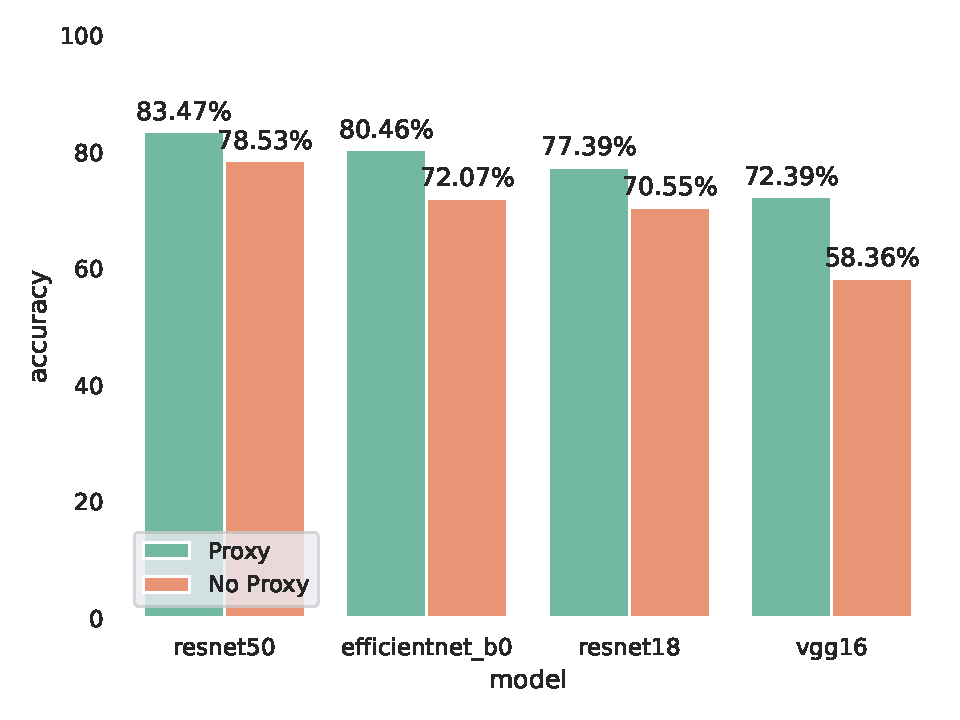
\includegraphics[width=1\textwidth]{results/tsing_results.pdf}
    \caption{Comparing Accuracies of models trained with and without Proxy Attention on the Tsing dataset}
    \label{fig:tsing_results}
\end{figure}

\subsection{Places256 Results}
This section shows the accuracies per model for the Places256 dataset. The results are shown in Figure \ref{fig:places256_results}. 
\begin{figure}[H]
    \centering
    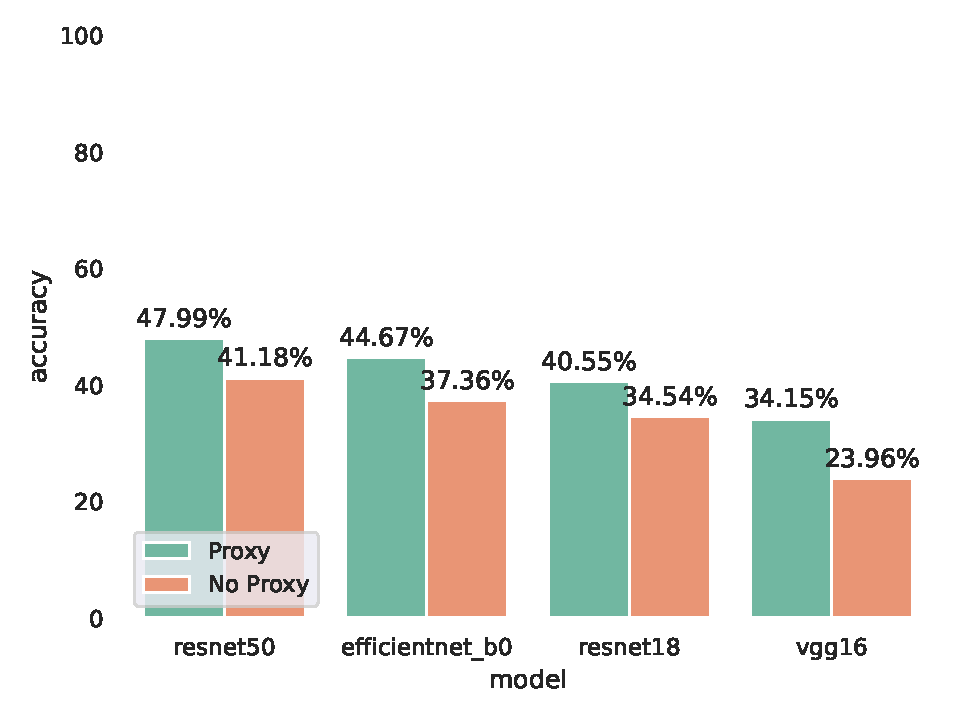
\includegraphics[width=1\textwidth]{results/places256_results.pdf}
    \caption{Comparing Accuracies of models trained with and without Proxy Attention on the Places256 dataset}
    \label{fig:places256_results}
\end{figure}

\subsection{Dogs Results}
This section shows the accuracies per model for the Dogs dataset. The results are shown in Figure \ref{fig:dogs_results}. 
\begin{figure}[H]
    \centering
    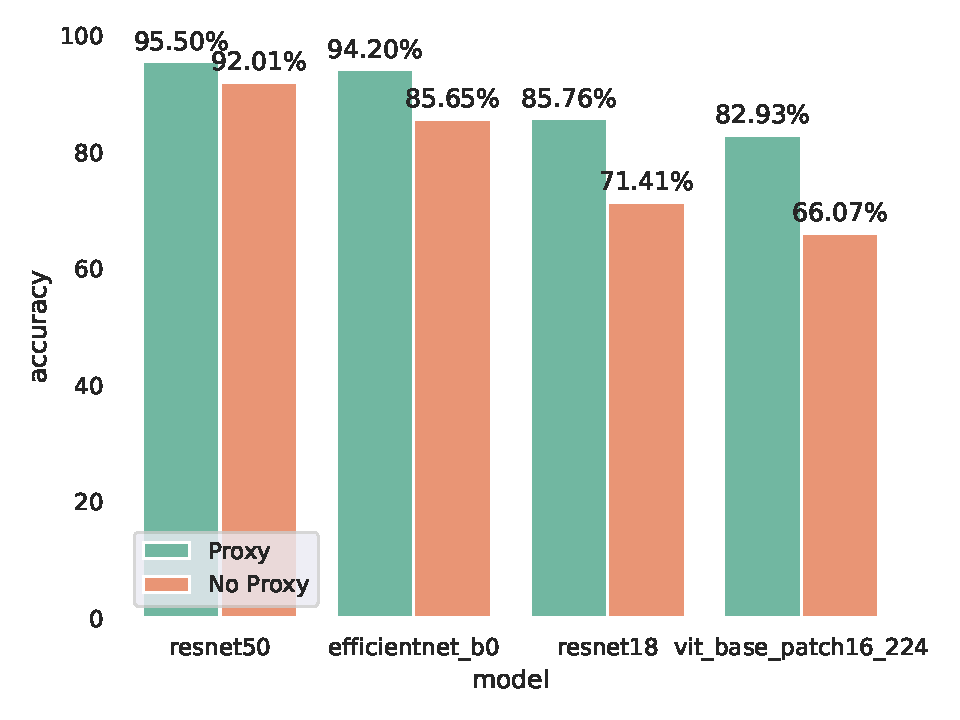
\includegraphics[width=1\textwidth]{results/dogs_results.pdf}
    \caption{Comparing Accuracies of models trained with and without Proxy Attention on the Dogs dataset}
    \label{fig:dogs_results}
\end{figure}

\subsection{Cifar100 Results}
This section shows the accuracies per model for the Cifar100 dataset. The results are shown in Figure \ref{fig:cifar100_results}. 
\begin{figure}[H]
    \centering
    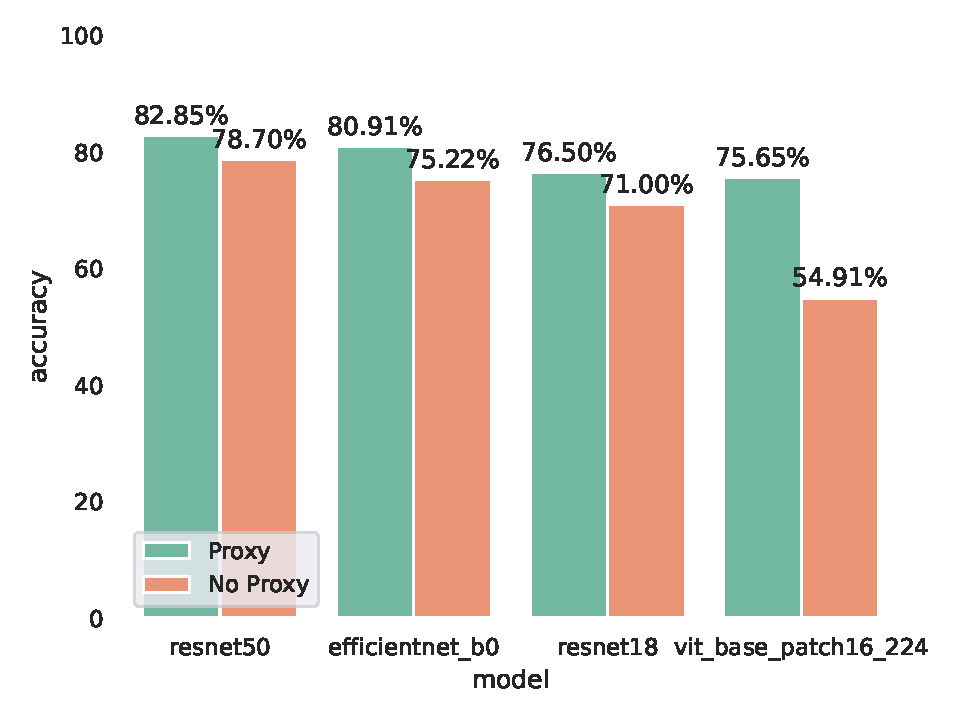
\includegraphics[width=1\textwidth]{results/cifar100_results.pdf}
    \caption{Comparing Accuracies of models trained with and without Proxy Attention on the Cifar100 dataset}
    \label{fig:cifar100_results}
\end{figure}

\subsection{Caltech101 Results}
This section shows the accuracies per model for the Caltech101 dataset. The results are shown in Figure \ref{fig:caltech101_results}. 
\begin{figure}[H]
    \centering
    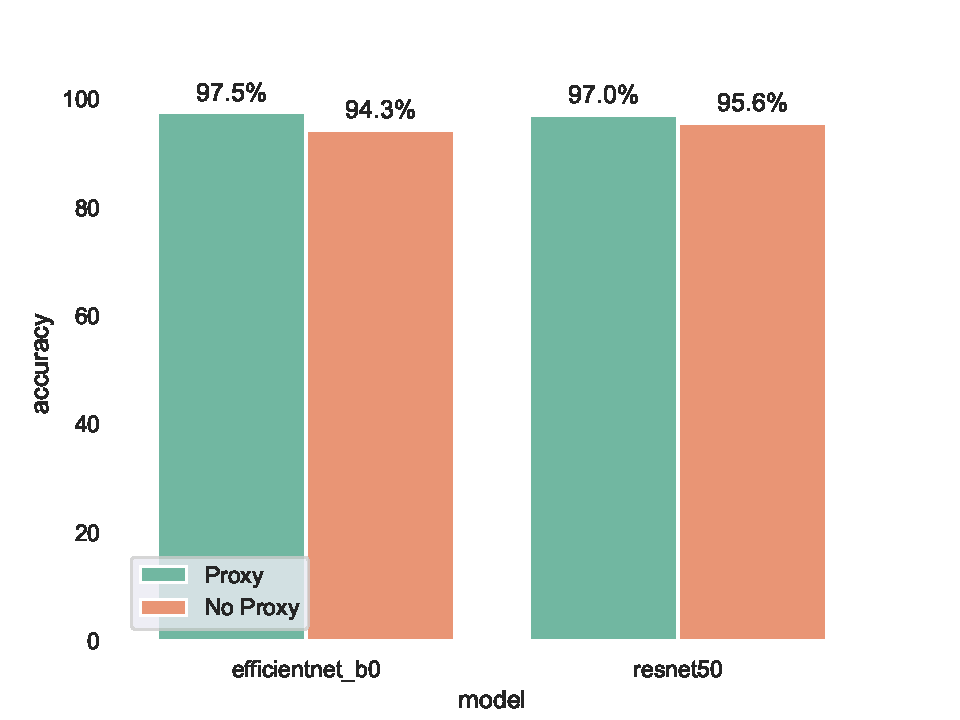
\includegraphics[width=1\textwidth]{results/caltech101_results.pdf}
    \caption{Comparing Accuracies of models trained with and without Proxy Attention on the Caltech101 dataset}
    \label{fig:caltech101_results}
\end{figure}

\subsection{Asl Results}
This section shows the accuracies per model for the Asl dataset. The results are shown in Figure \ref{fig:asl_results}. 
\begin{figure}[H]
    \centering
    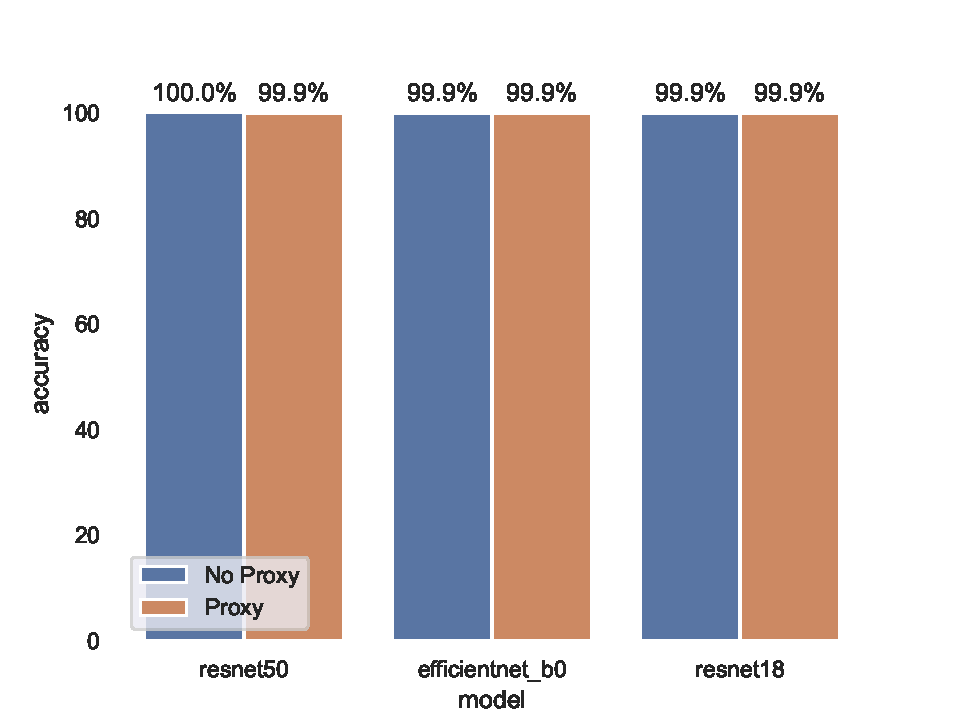
\includegraphics[width=1\textwidth]{results/asl_results.pdf}
    \caption{Comparing Accuracies of models trained with and without Proxy Attention on the Asl dataset}
    \label{fig:asl_results}
\end{figure}

\subsection{Plantdisease Results}
This section shows the accuracies per model for the Plantdisease dataset. The results are shown in Figure \ref{fig:plantdisease_results}. 
\begin{figure}[H]
    \centering
    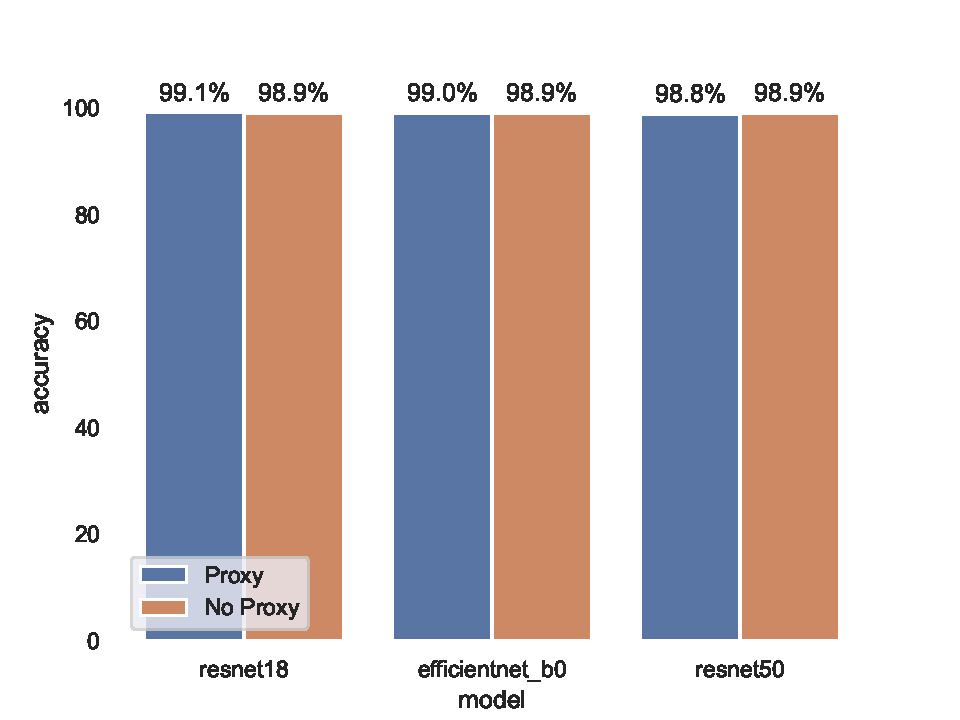
\includegraphics[width=1\textwidth]{results/plantdisease_results.pdf}
    \caption{Comparing Accuracies of models trained with and without Proxy Attention on the Plantdisease dataset}
    \label{fig:plantdisease_results}
\end{figure}


\subsection{Results Grouped By Schedule}
This section explores the validation accuracy obtained for different step schedules. The results are shown in Figure \ref{fig:schedresnet50_results}. 
\begin{figure}[H]
    \centering
    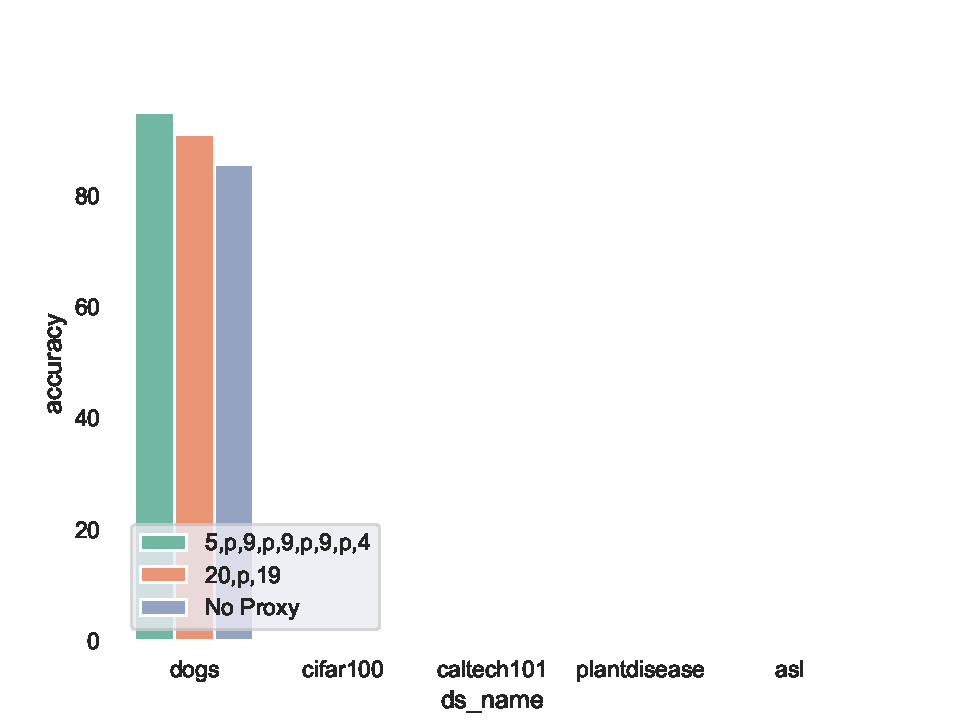
\includegraphics[width=1\textwidth]{results/schedule_resnet50.pdf}
    \caption{Comparing Accuracies of models trained with and without Proxy Attention on the ResNet50 \cite{heDeepResidualLearning2016} architecture for different step schedules}.
    \label{fig:schedresnet50_results}
\end{figure}

\subsection{Results Grouped By Proxy Threshold}
This section explores the validation accuracy obtained for different Proxy thresholds. The results are shown in Figure \ref{fig:proxy_threshold}. 
\begin{figure}[H]
    \centering
    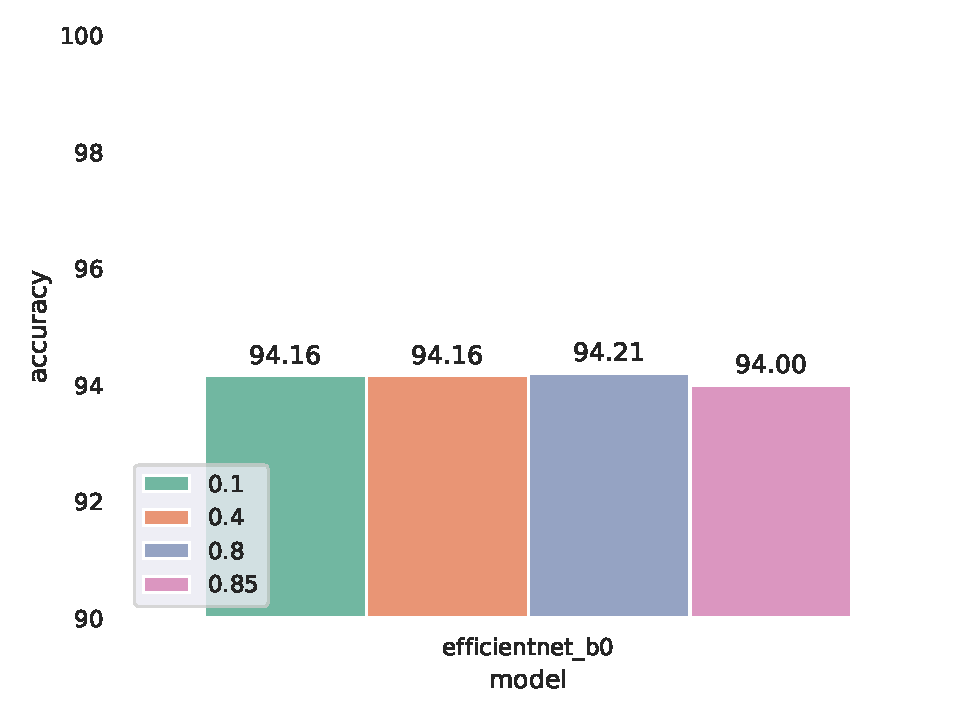
\includegraphics[width=1\textwidth]{results/proxy_threshold_results.pdf}
    \caption{Comparing Accuracies of EfficientNetB0 \cite{tanEfficientnetRethinkingModel2019} trained with Proxy Attention on the Stanford Dogs dataset\cite{khoslaNovelDatasetFineGrained} for different Proxy Thresholds}
    \label{fig:proxy_threshold}
\end{figure}

\begin{figure}[H]
    \centering
    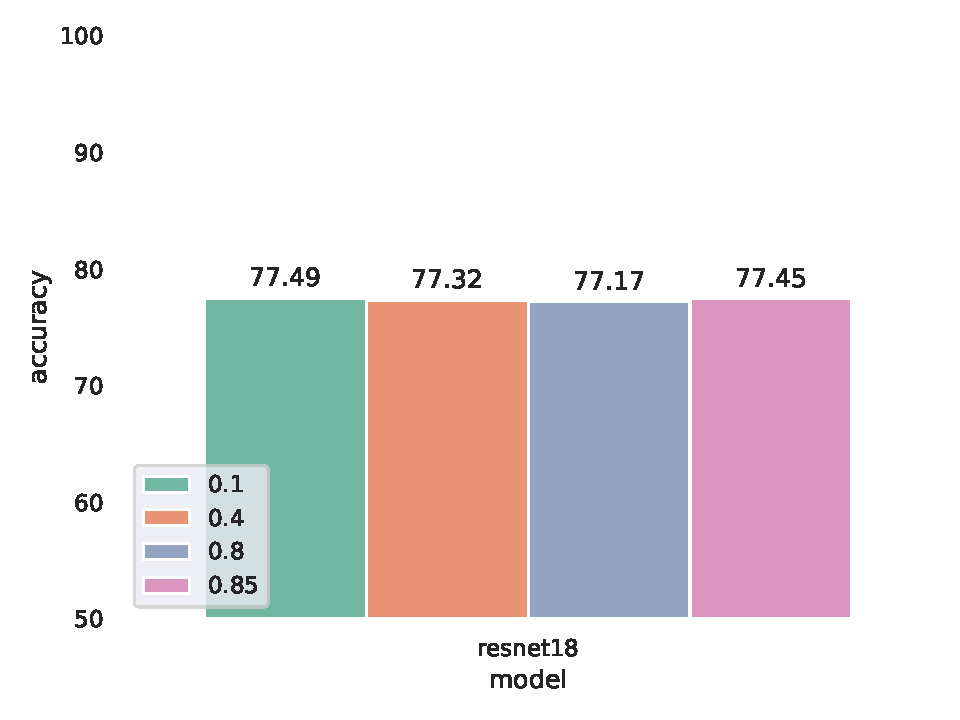
\includegraphics[width=1\textwidth]{results/proxy_threshold_results_tsing.pdf}
    \caption{Comparing Accuracies of Resnet18 \cite{heDeepResidualLearning2016} trained with Proxy Attention on the Tsinghua Dogs Dataset \cite{zouNewDatasetDog2020} for different Proxy Thresholds}
    \label{fig:proxy_threshold2}
\end{figure}

\subsection{Results Grouped By Proxy Image Weight}
This section explores the validation accuracy obtained for different Proxy image weights. The results are shown in Figure \ref{fig:proxy_weight}. 

\begin{figure}[H]
    \centering
    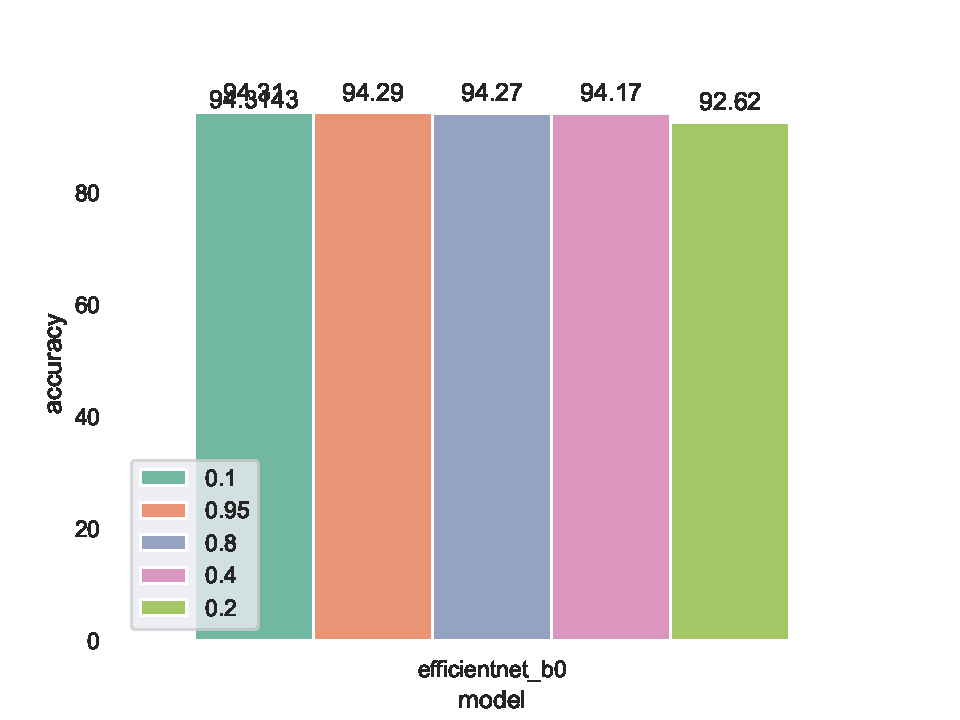
\includegraphics[width=1\textwidth]{results/proxy_weight_results.pdf}
    \caption{Comparing Accuracies of EfficientNetB0 \cite{tanEfficientnetRethinkingModel2019} trained with Proxy Attention on the Stanford Dogs dataset\cite{khoslaNovelDatasetFineGrained} for different Proxy Image Weights}
    \label{fig:proxy_weight}
\end{figure}

\begin{figure}[H]
    \centering
    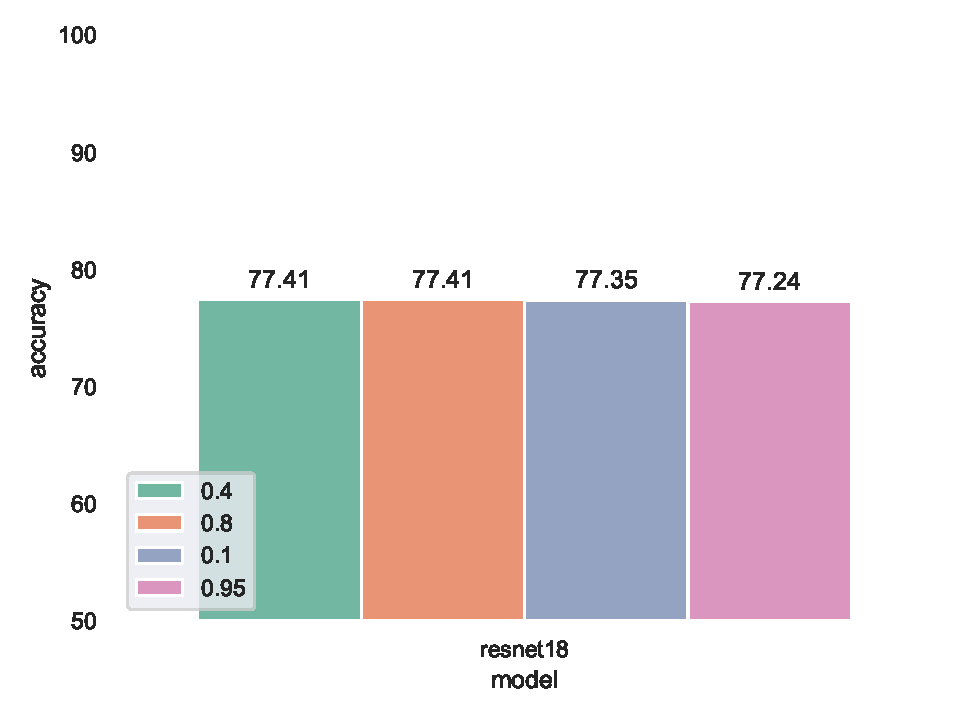
\includegraphics[width=1\textwidth]{results/proxy_weight_results_tsing.pdf}
    \caption{Comparing Accuracies of Resnet18 \cite{heDeepResidualLearning2016} trained with Proxy Attention on the Tsinghua Dogs Dataset \cite{zouNewDatasetDog2020} for different Proxy Image Weights}
    \label{fig:proxy_weight2}
\end{figure}

\subsection{Results Grouped By Proxy Image Subset}
This section explores the validation accuracy obtained for different Proxy image subsets. The results are shown in Figure \ref{fig:proxy_subset}.

\begin{figure}[H]
    \centering
    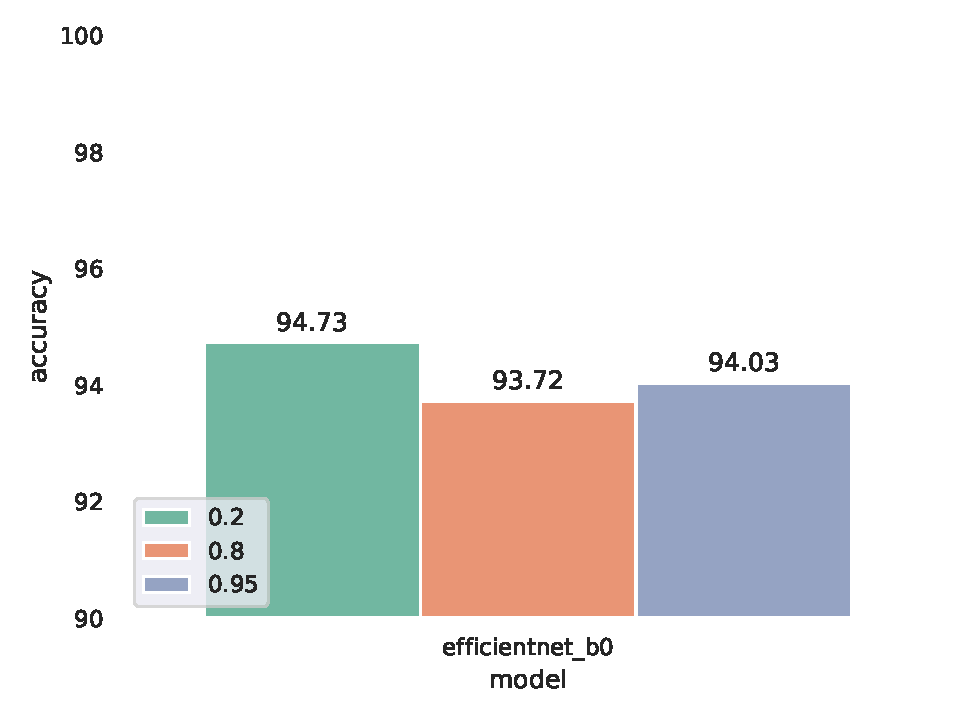
\includegraphics[width=1\textwidth]{results/proxy_subset_attention_results.pdf}
    \caption{Comparing Accuracies of EfficientNetB0 \cite{tanEfficientnetRethinkingModel2019} trained with Proxy Attention on the Stanford Dogs dataset\cite{khoslaNovelDatasetFineGrained} for different Proxy Image Subsets}
    \label{fig:proxy_subset}
\end{figure}

\begin{figure}[H]
    \centering
    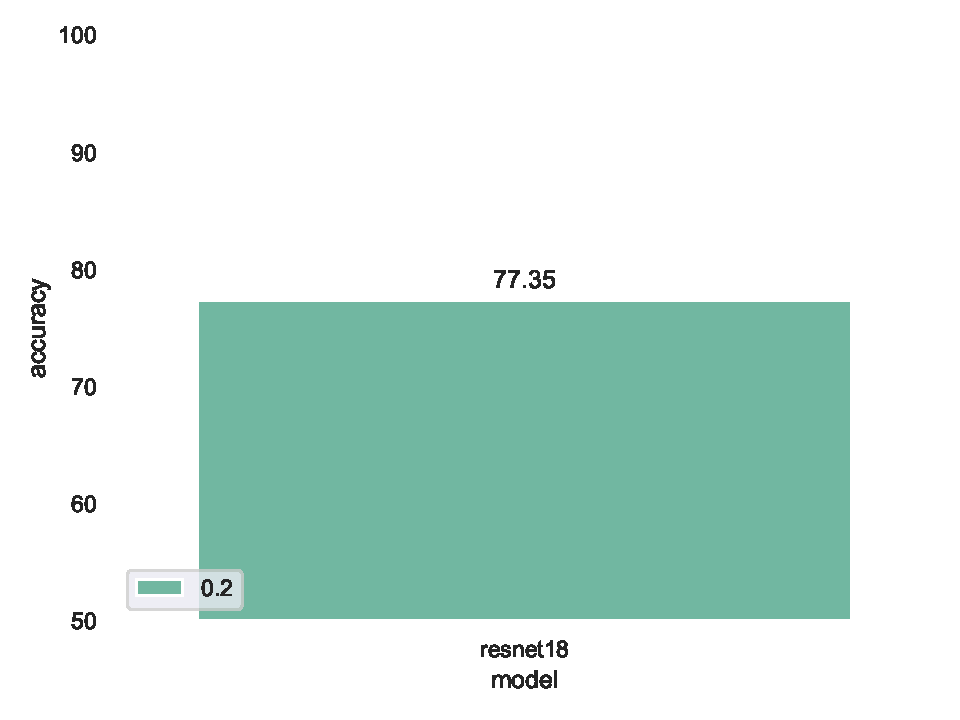
\includegraphics[width=1\textwidth]{results/proxy_subset_results_tsing.pdf}
    \caption{Comparing Accuracies of Resnet18 \cite{heDeepResidualLearning2016} trained with Proxy Attention on the Tsinghua Dogs Dataset \cite{zouNewDatasetDog2020} for different Proxy Image Subsets}
    \label{fig:proxy_subset2}
\end{figure}


\section{Explanability}
This section explores the explainability of the models for different hyperparameters and datasets by using a trained model to generate attention maps for a given input image. The attention maps are compared between the same network (with the same hyperparameters) trained with and without Proxy Attention.

\subsection{CIFAR 100, ResNet18, EigenGradCAM}

    \begin{figure}[H]
        \centering
        \begin{subfigure}[b]{1\textwidth}
            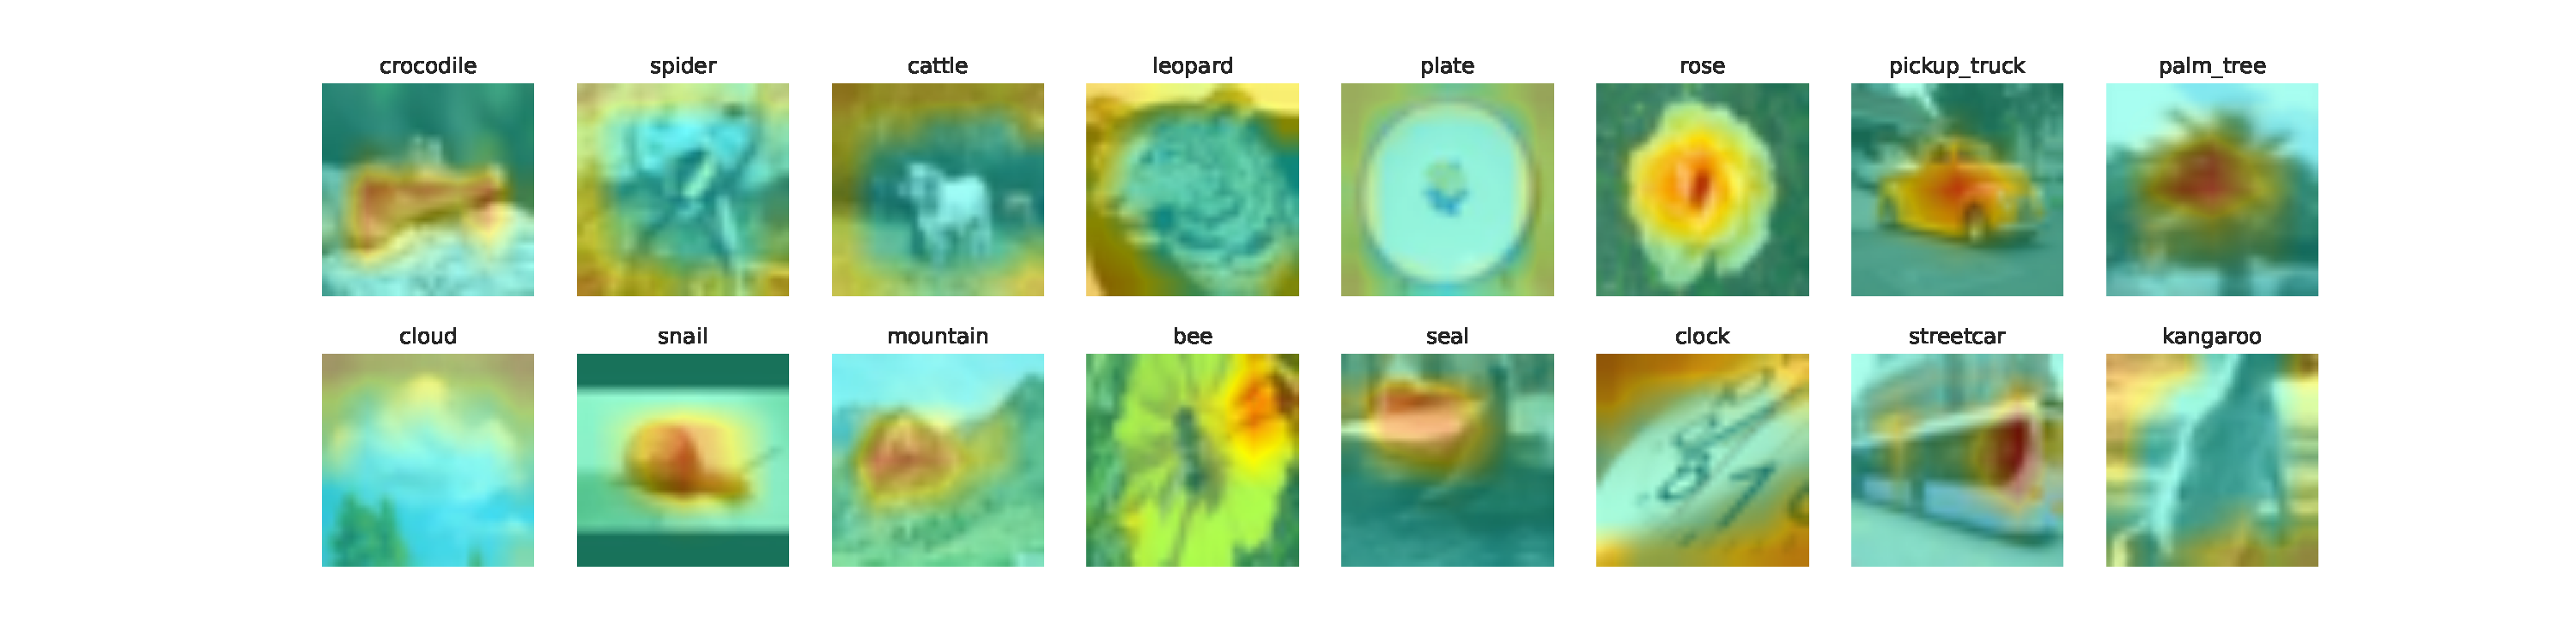
\includegraphics[width=\textwidth]{images/cifar100_resnet18_noproxy_0.pdf}
            \caption{Without Proxy Attention}
        \end{subfigure}
        \hfill
        \begin{subfigure}[b]{1\textwidth}
            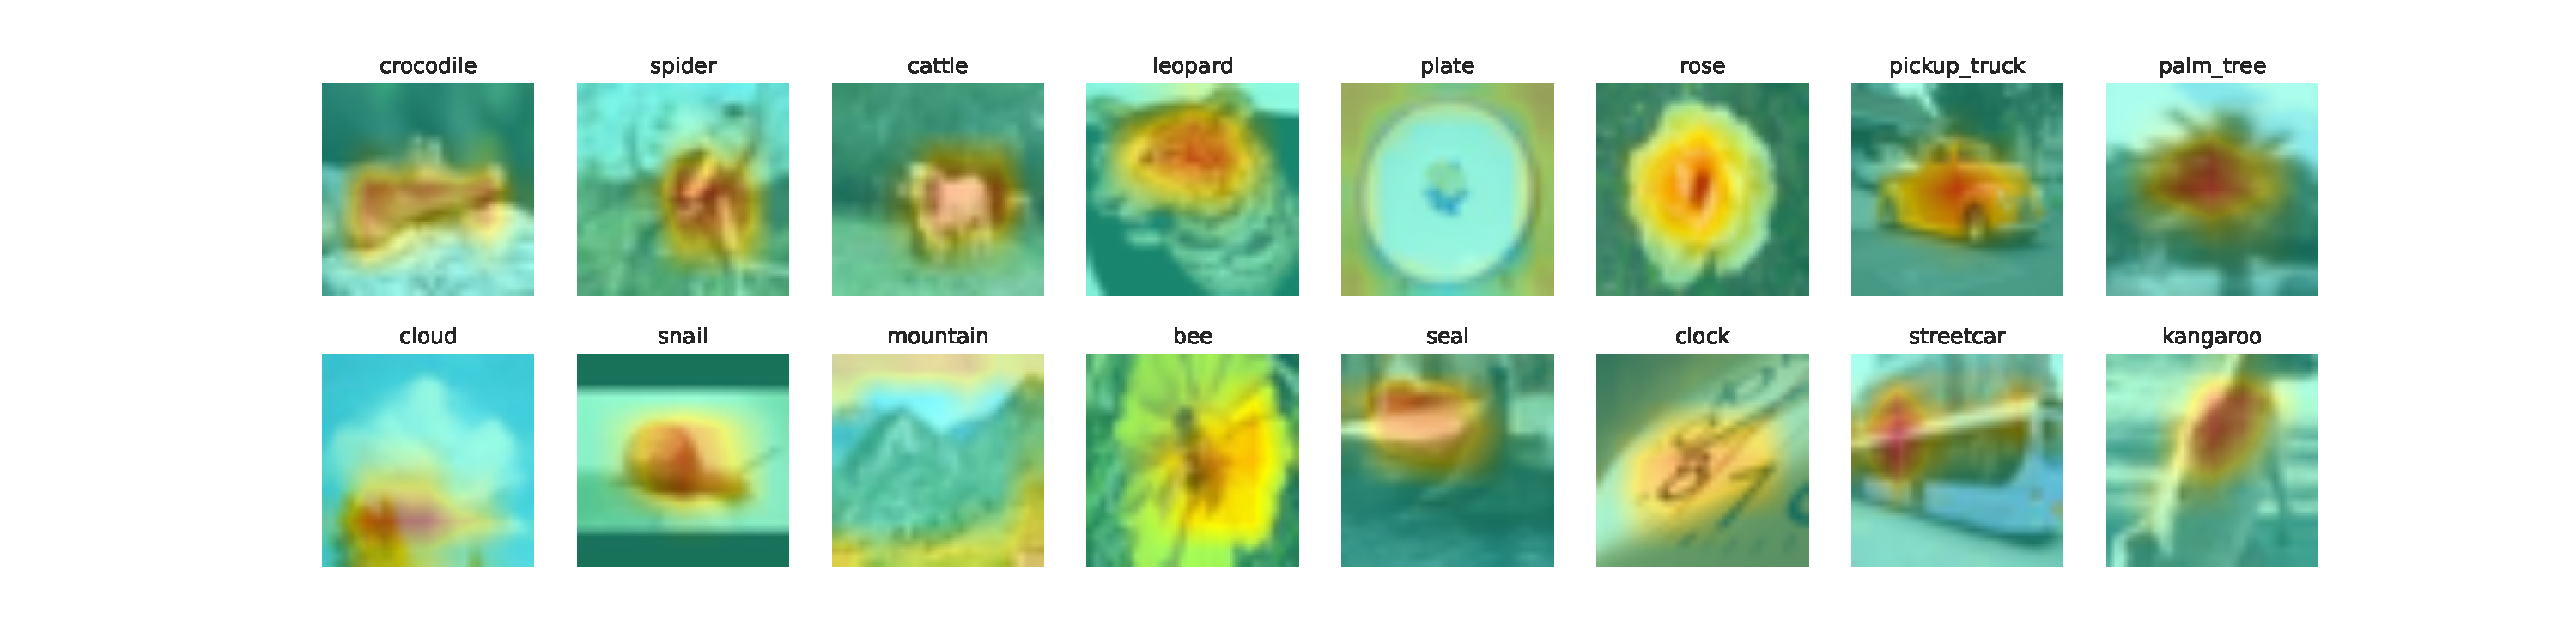
\includegraphics[width=\textwidth]{images/cifar100_resnet18_proxy_0.pdf}
            \caption{With Proxy Attention}
        \end{subfigure}
        \caption{Comparison of attention maps generated by resnet18 trained with and without Proxy Attention on the cifar100 dataset}
    \end{figure}
    

    \begin{figure}[H]
        \centering
        \begin{subfigure}[b]{1\textwidth}
            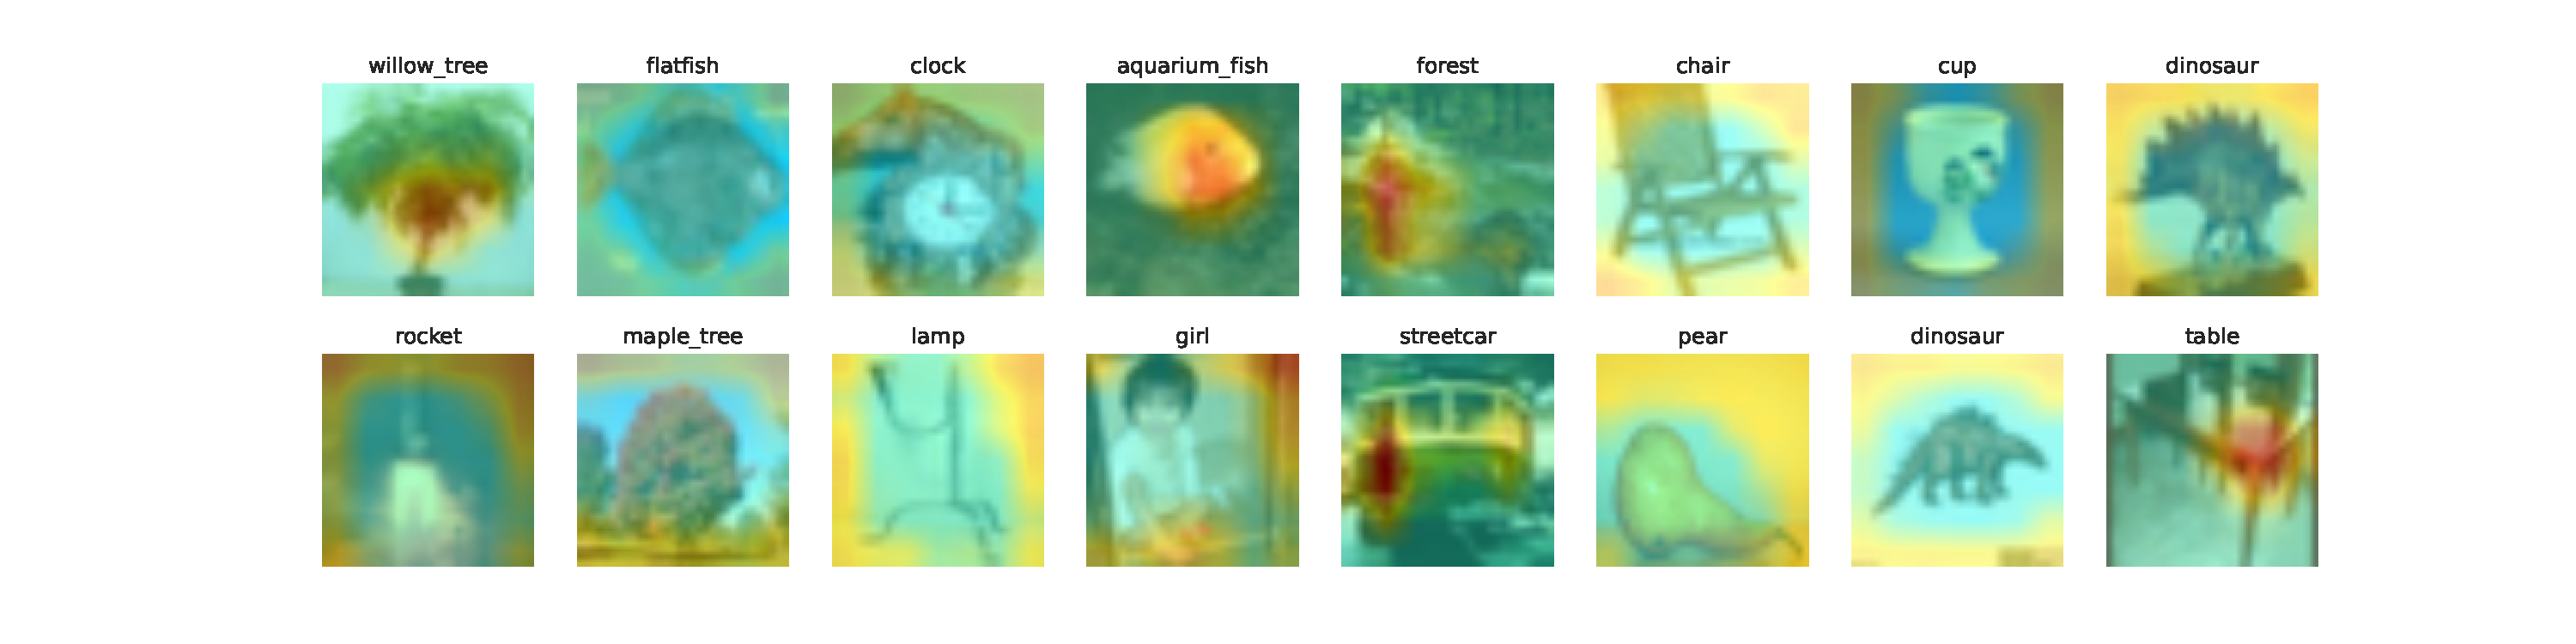
\includegraphics[width=\textwidth]{images/cifar100_resnet18_noproxy_1.pdf}
            \caption{Without Proxy Attention}
        \end{subfigure}
        \hfill
        \begin{subfigure}[b]{1\textwidth}
            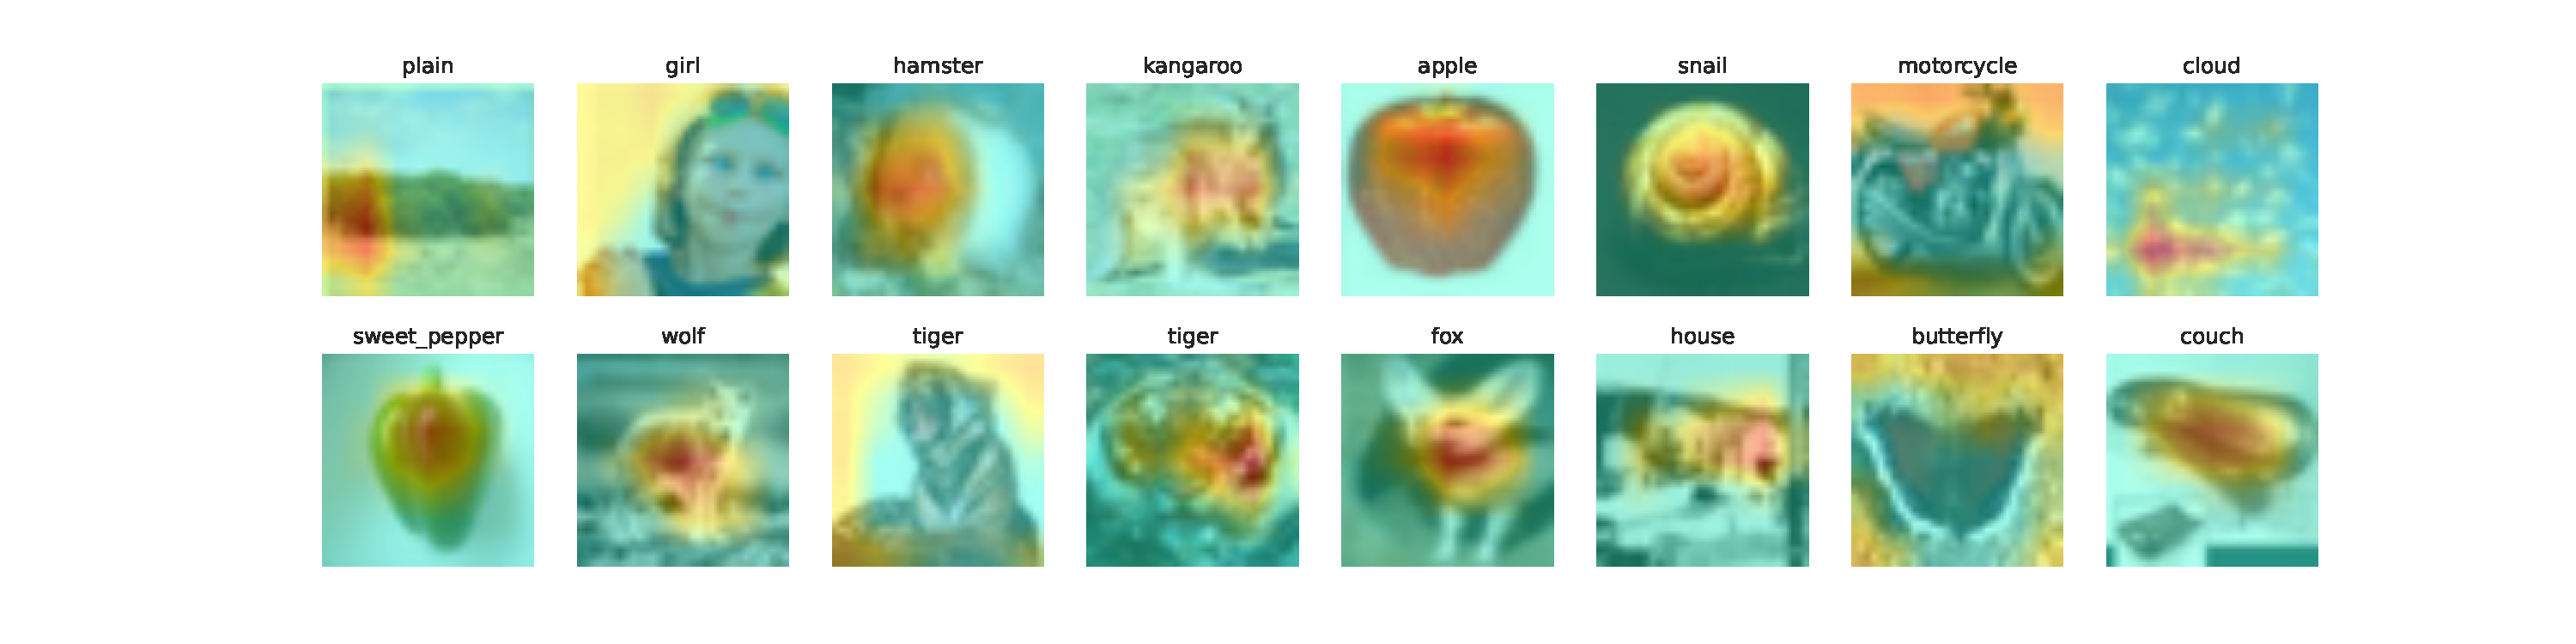
\includegraphics[width=\textwidth]{images/cifar100_resnet18_proxy_1.pdf}
            \caption{With Proxy Attention}
        \end{subfigure}
        \caption{Comparison of attention maps generated by resnet18 trained with and without Proxy Attention on the cifar100 dataset}
    \end{figure}
    

    \begin{figure}[H]
        \centering
        \begin{subfigure}[b]{1\textwidth}
            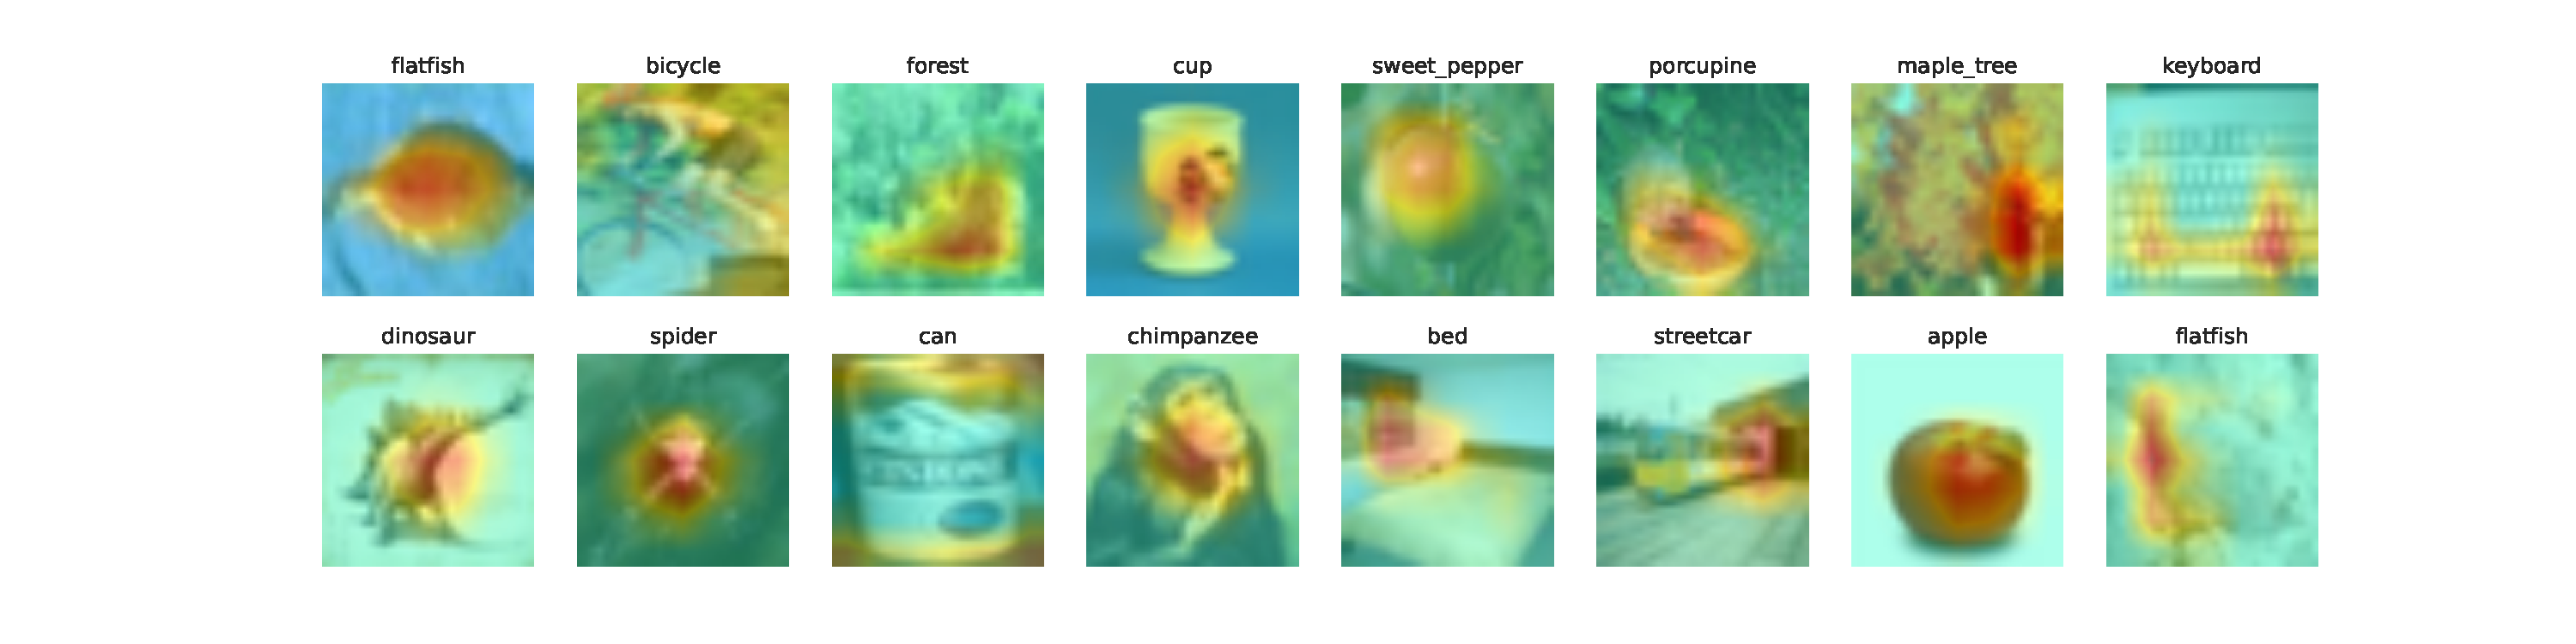
\includegraphics[width=\textwidth]{images/cifar100_resnet18_noproxy_2.pdf}
            \caption{Without Proxy Attention}
        \end{subfigure}
        \hfill
        \begin{subfigure}[b]{1\textwidth}
            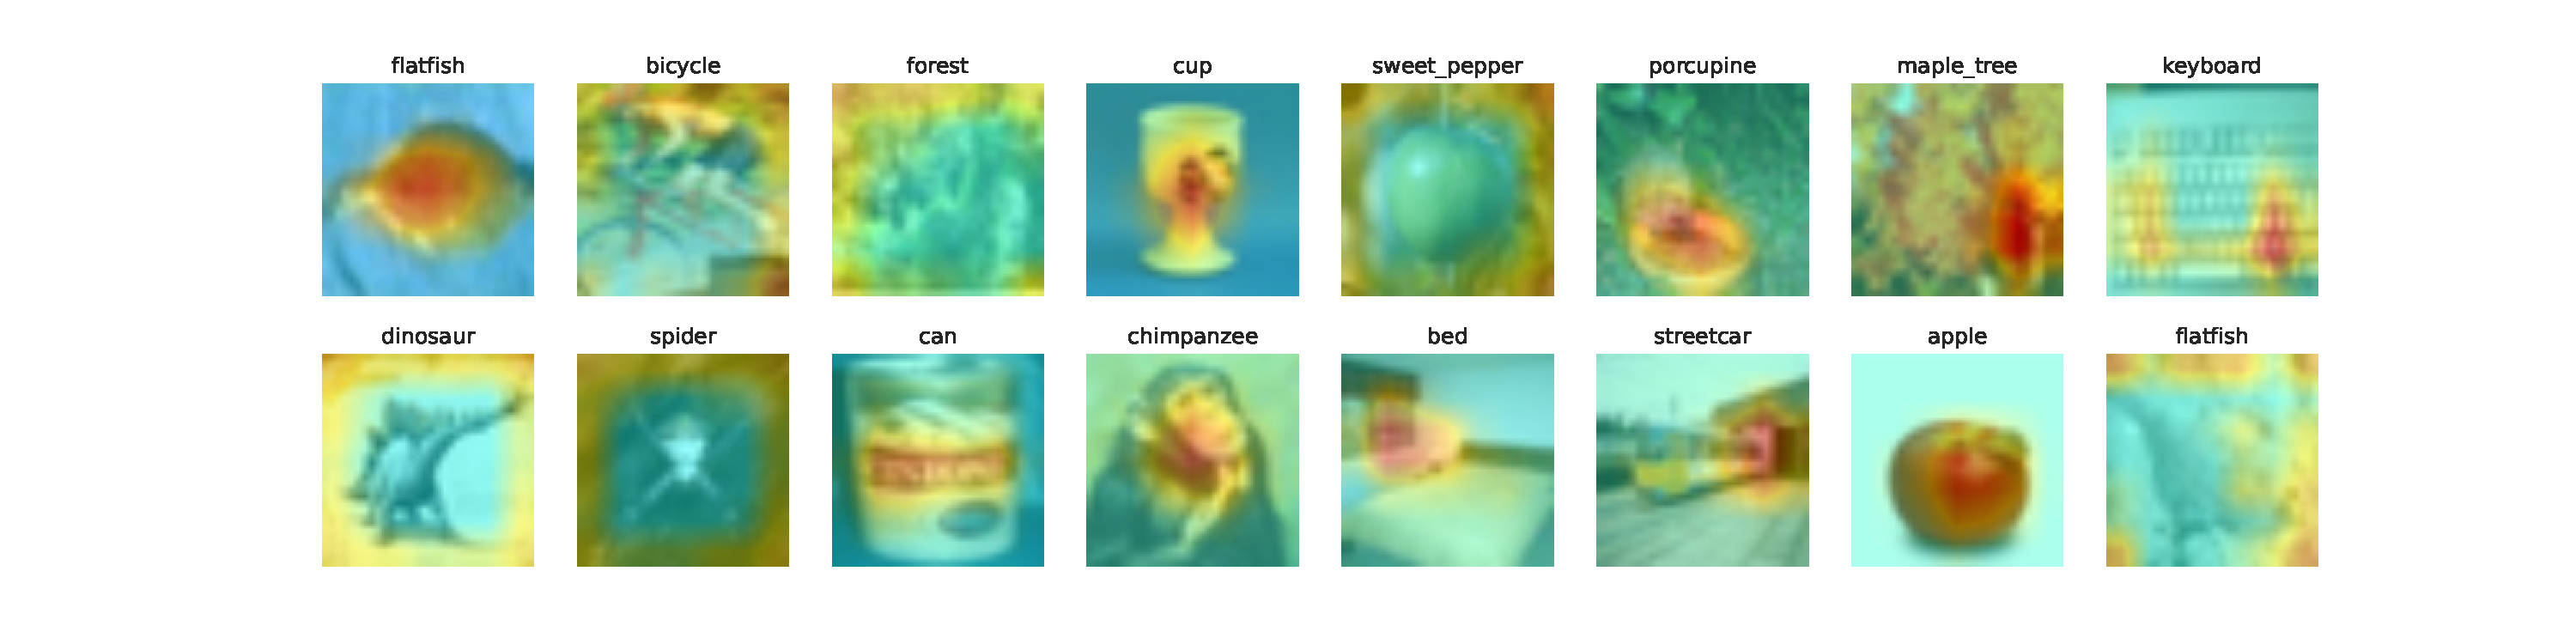
\includegraphics[width=\textwidth]{images/cifar100_resnet18_proxy_2.pdf}
            \caption{With Proxy Attention}
        \end{subfigure}
        \caption{Comparison of attention maps generated by resnet18 trained with and without Proxy Attention on the cifar100 dataset}
    \end{figure}
    

    \begin{figure}[H]
        \centering
        \begin{subfigure}[b]{1\textwidth}
            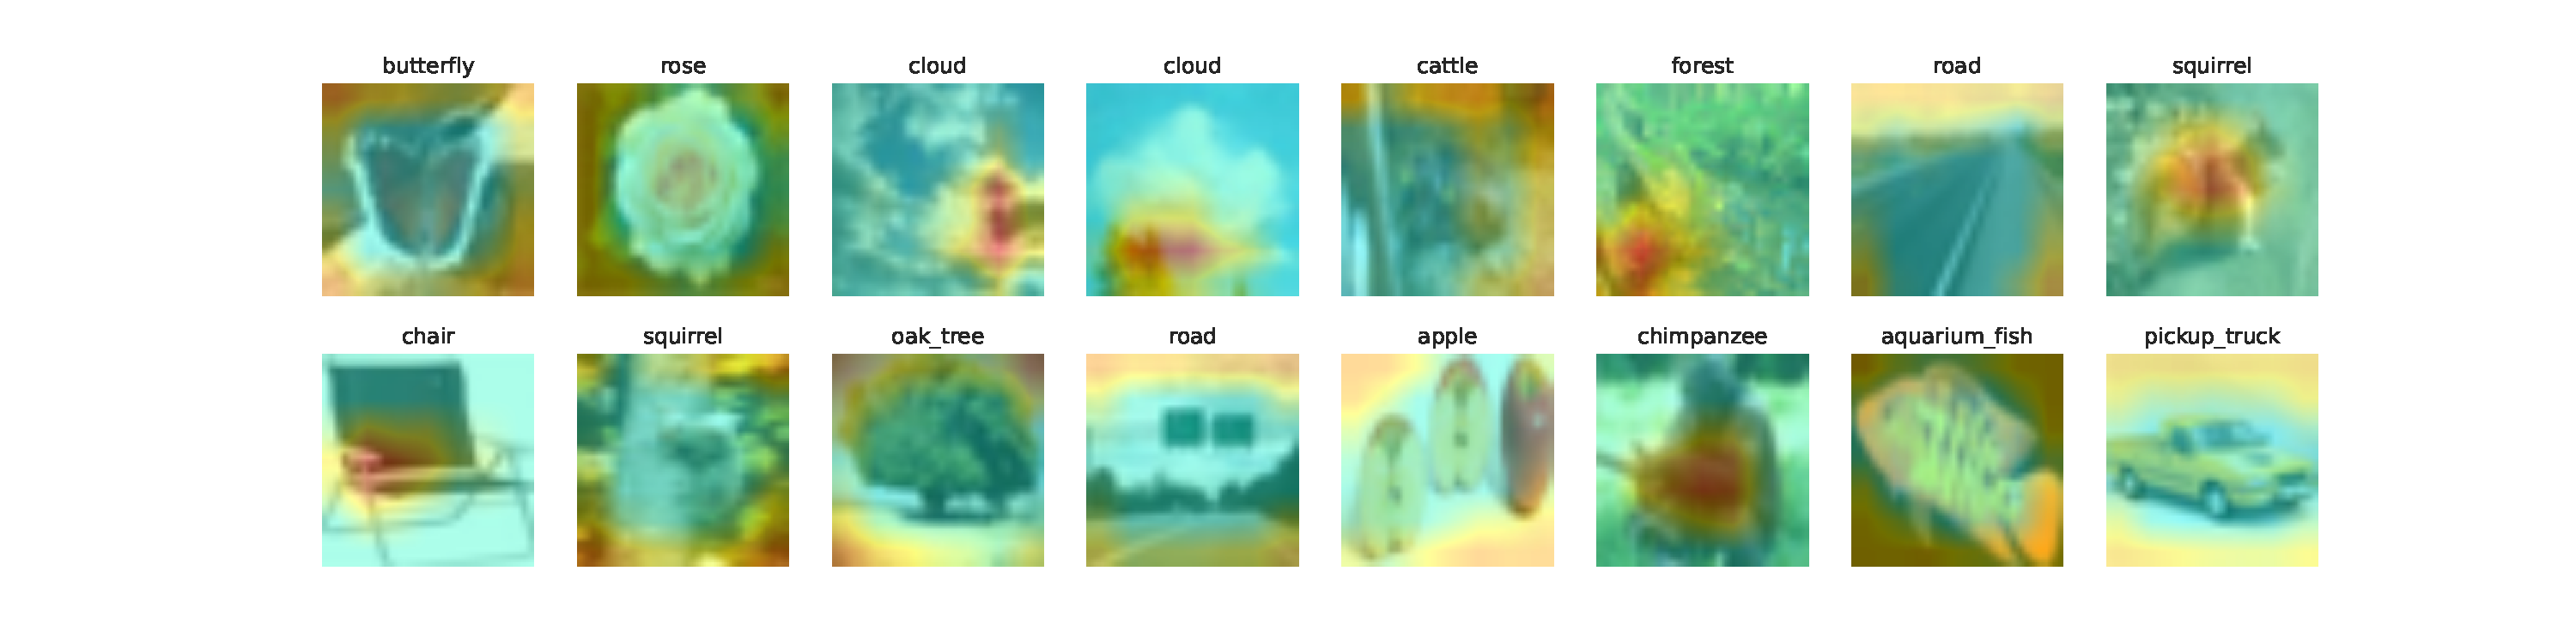
\includegraphics[width=\textwidth]{images/cifar100_resnet18_noproxy_3.pdf}
            \caption{Without Proxy Attention}
        \end{subfigure}
        \hfill
        \begin{subfigure}[b]{1\textwidth}
            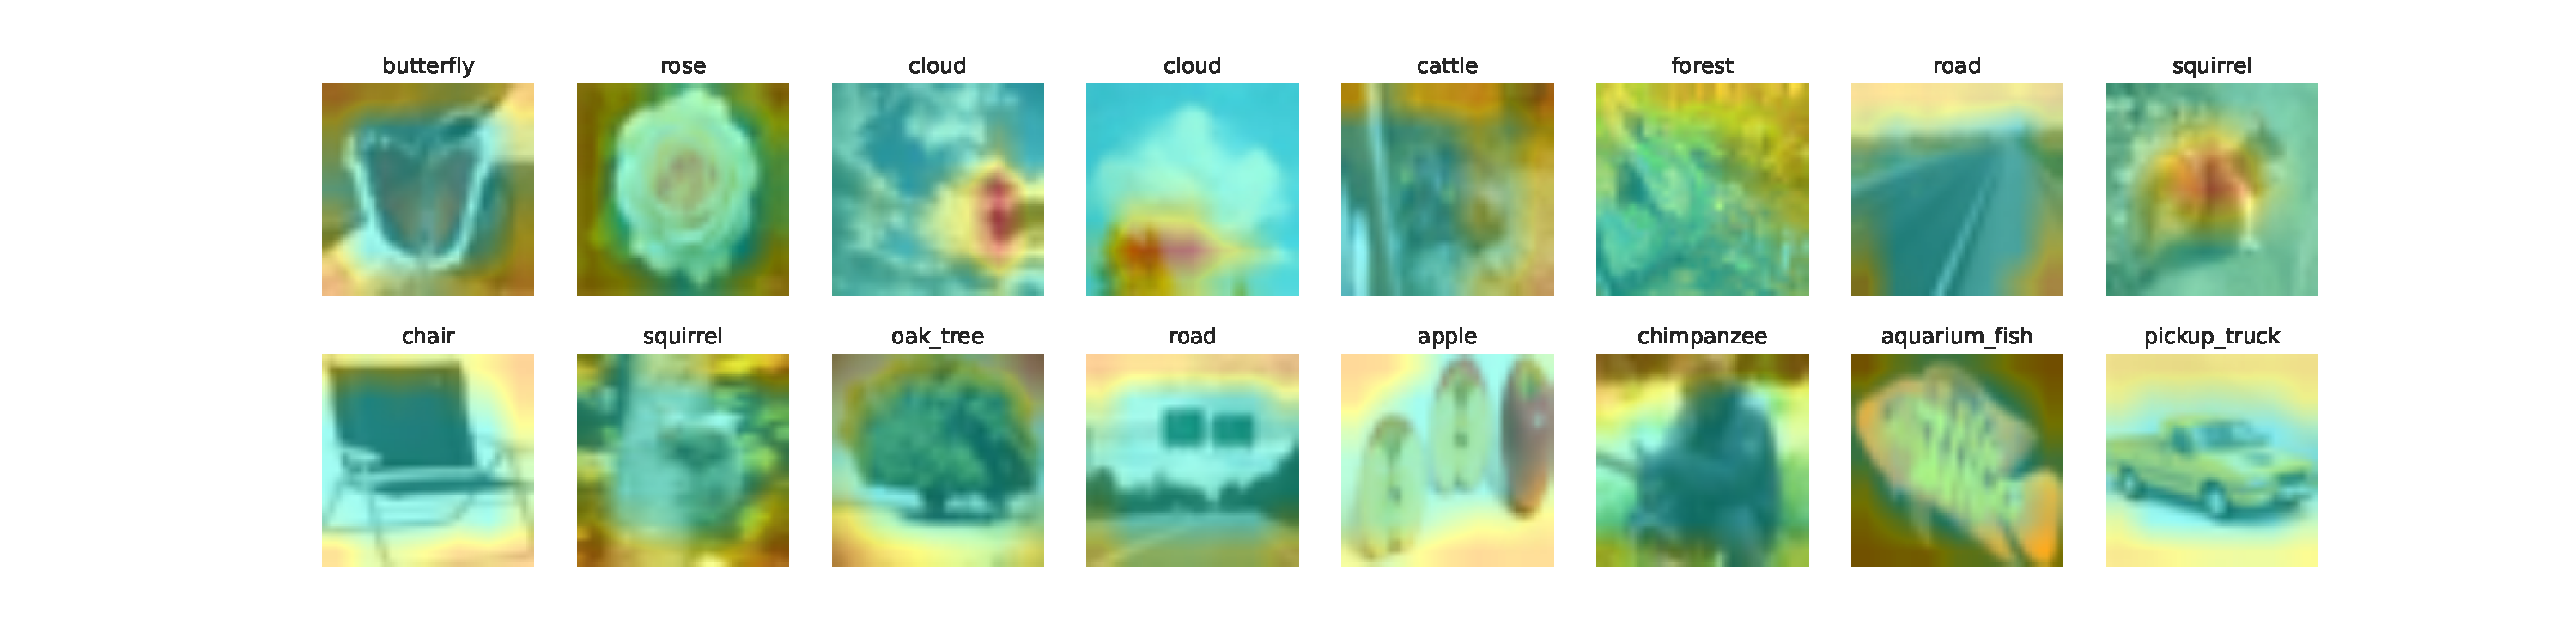
\includegraphics[width=\textwidth]{images/cifar100_resnet18_proxy_3.pdf}
            \caption{With Proxy Attention}
        \end{subfigure}
        \caption{Comparison of attention maps generated by resnet18 trained with and without Proxy Attention on the cifar100 dataset}
    \end{figure}
    


\subsection{CIFAR 100, EfficientNetB0, EigenGradCAM}

    \begin{figure}[H]
        \centering
        \begin{subfigure}[b]{1\textwidth}
            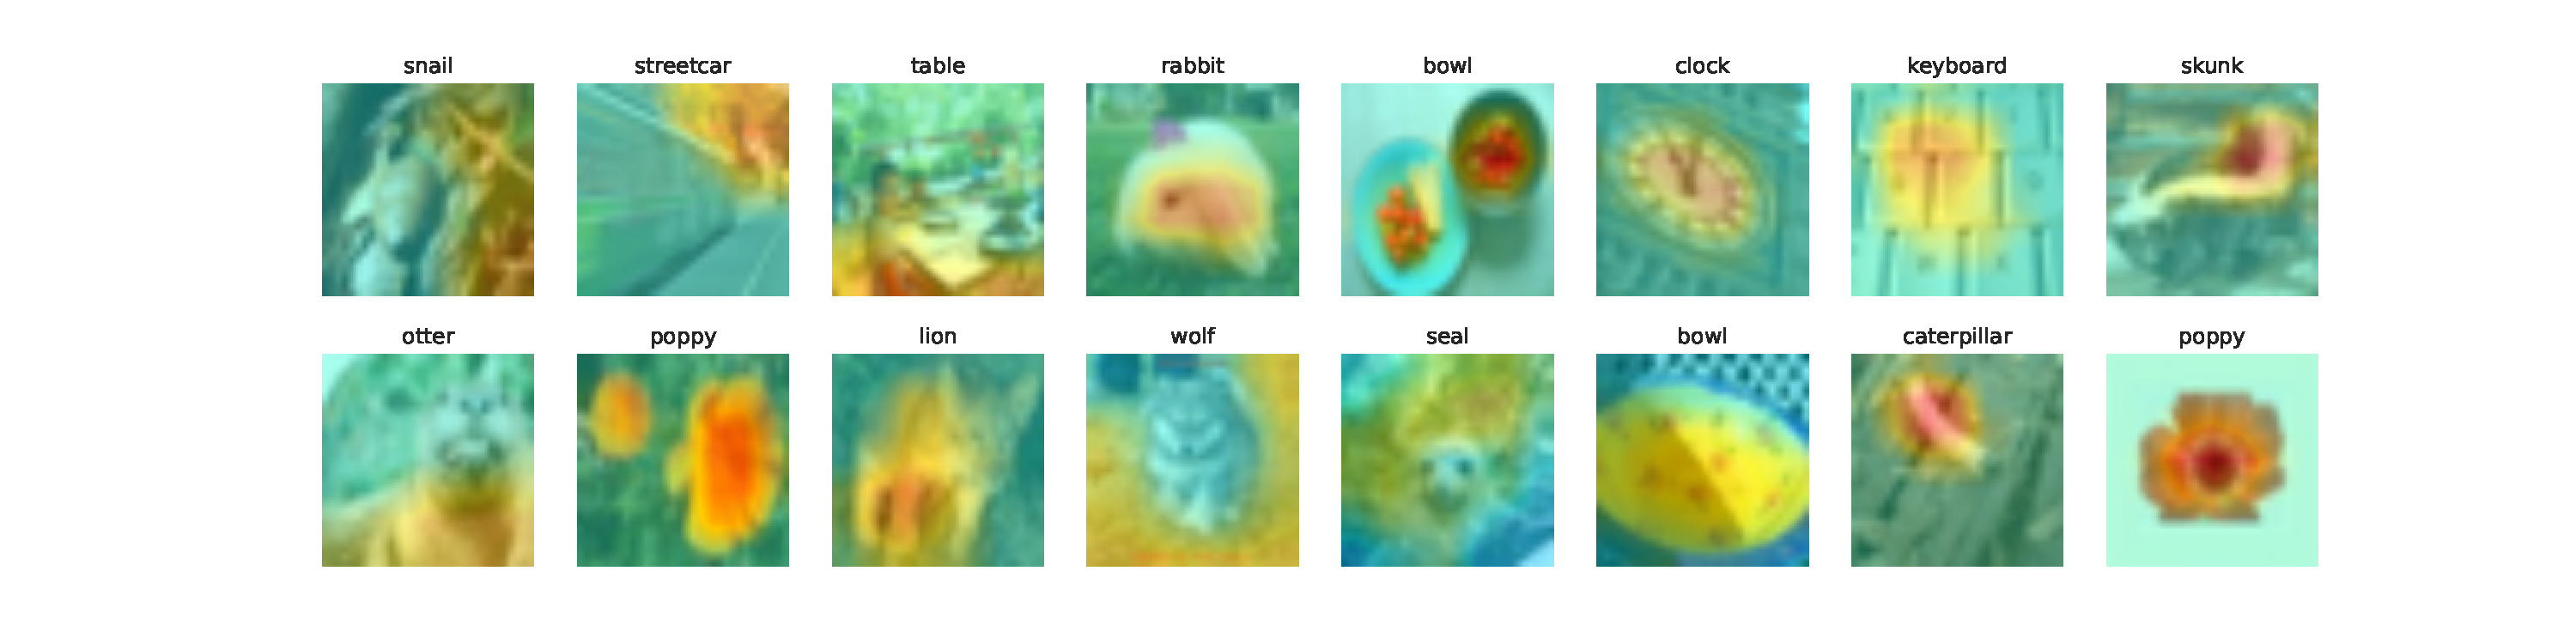
\includegraphics[width=\textwidth]{images/cifar100_efficientnet_b0_noproxy_0.pdf}
            \caption{Without Proxy Attention}
        \end{subfigure}
        \hfill
        \begin{subfigure}[b]{1\textwidth}
            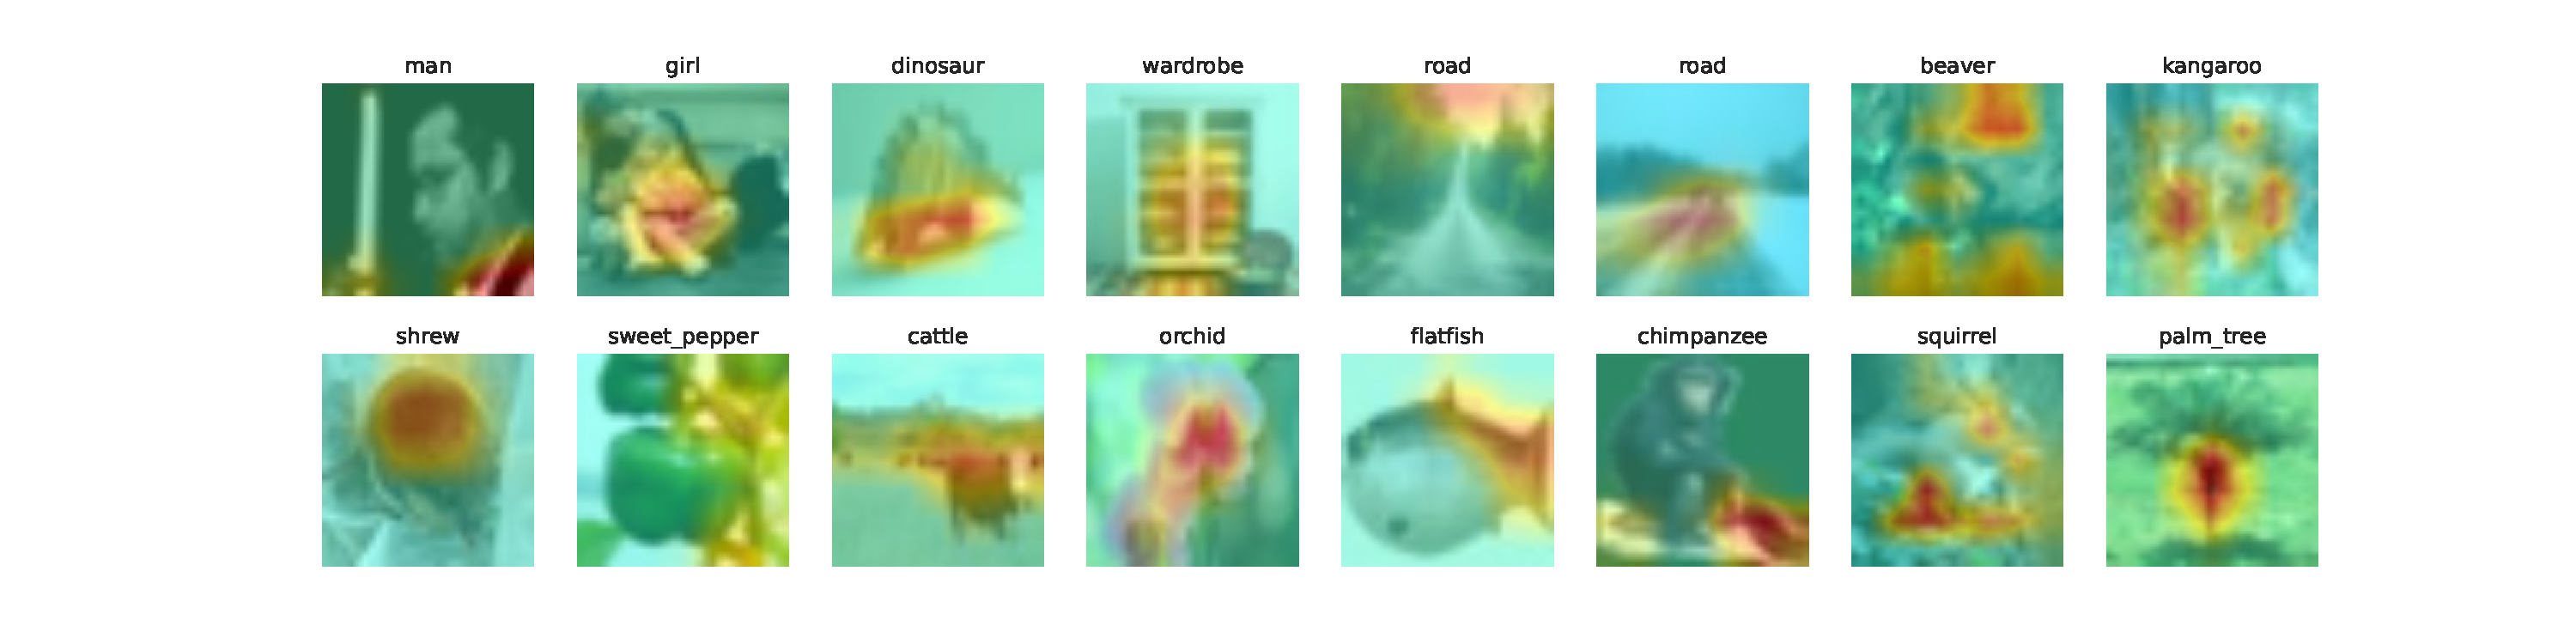
\includegraphics[width=\textwidth]{images/cifar100_efficientnet_b0_proxy_0.pdf}
            \caption{With Proxy Attention}
        \end{subfigure}
        \caption{Comparison of attention maps generated by efficientnet\_b0 trained with and without Proxy Attention on the cifar100 dataset}
    \end{figure}
    

    \begin{figure}[H]
        \centering
        \begin{subfigure}[b]{1\textwidth}
            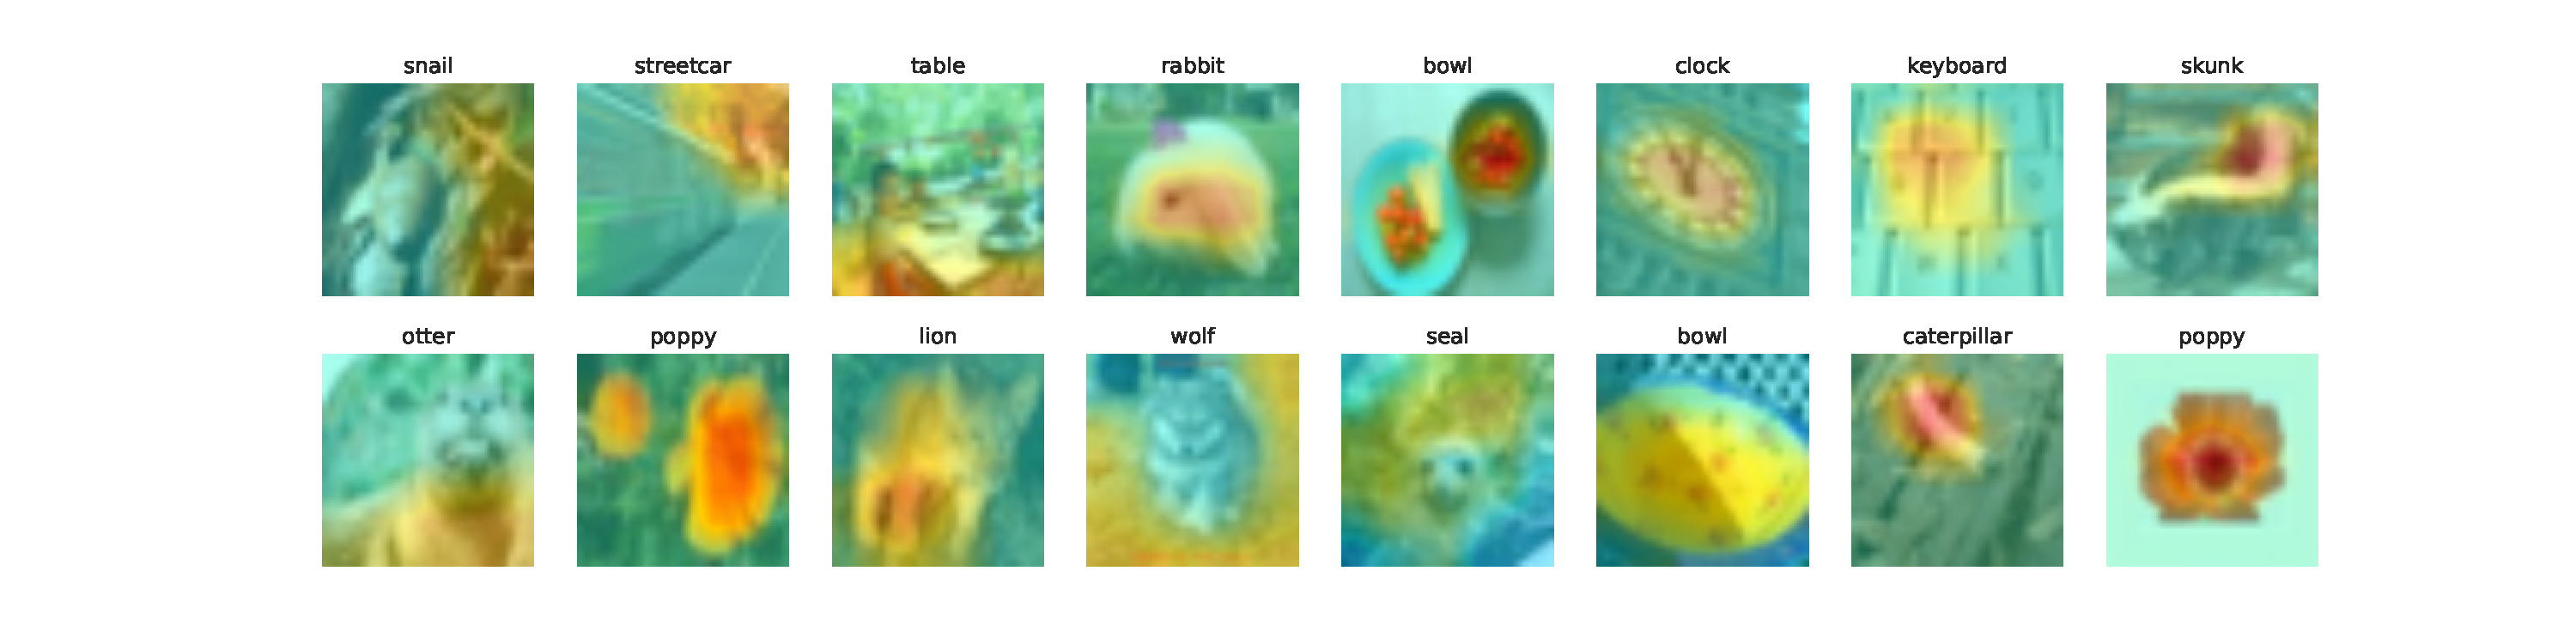
\includegraphics[width=\textwidth]{images/cifar100_efficientnet_b0_noproxy_0.pdf}
            \caption{Without Proxy Attention}
        \end{subfigure}
        \hfill
        \begin{subfigure}[b]{1\textwidth}
            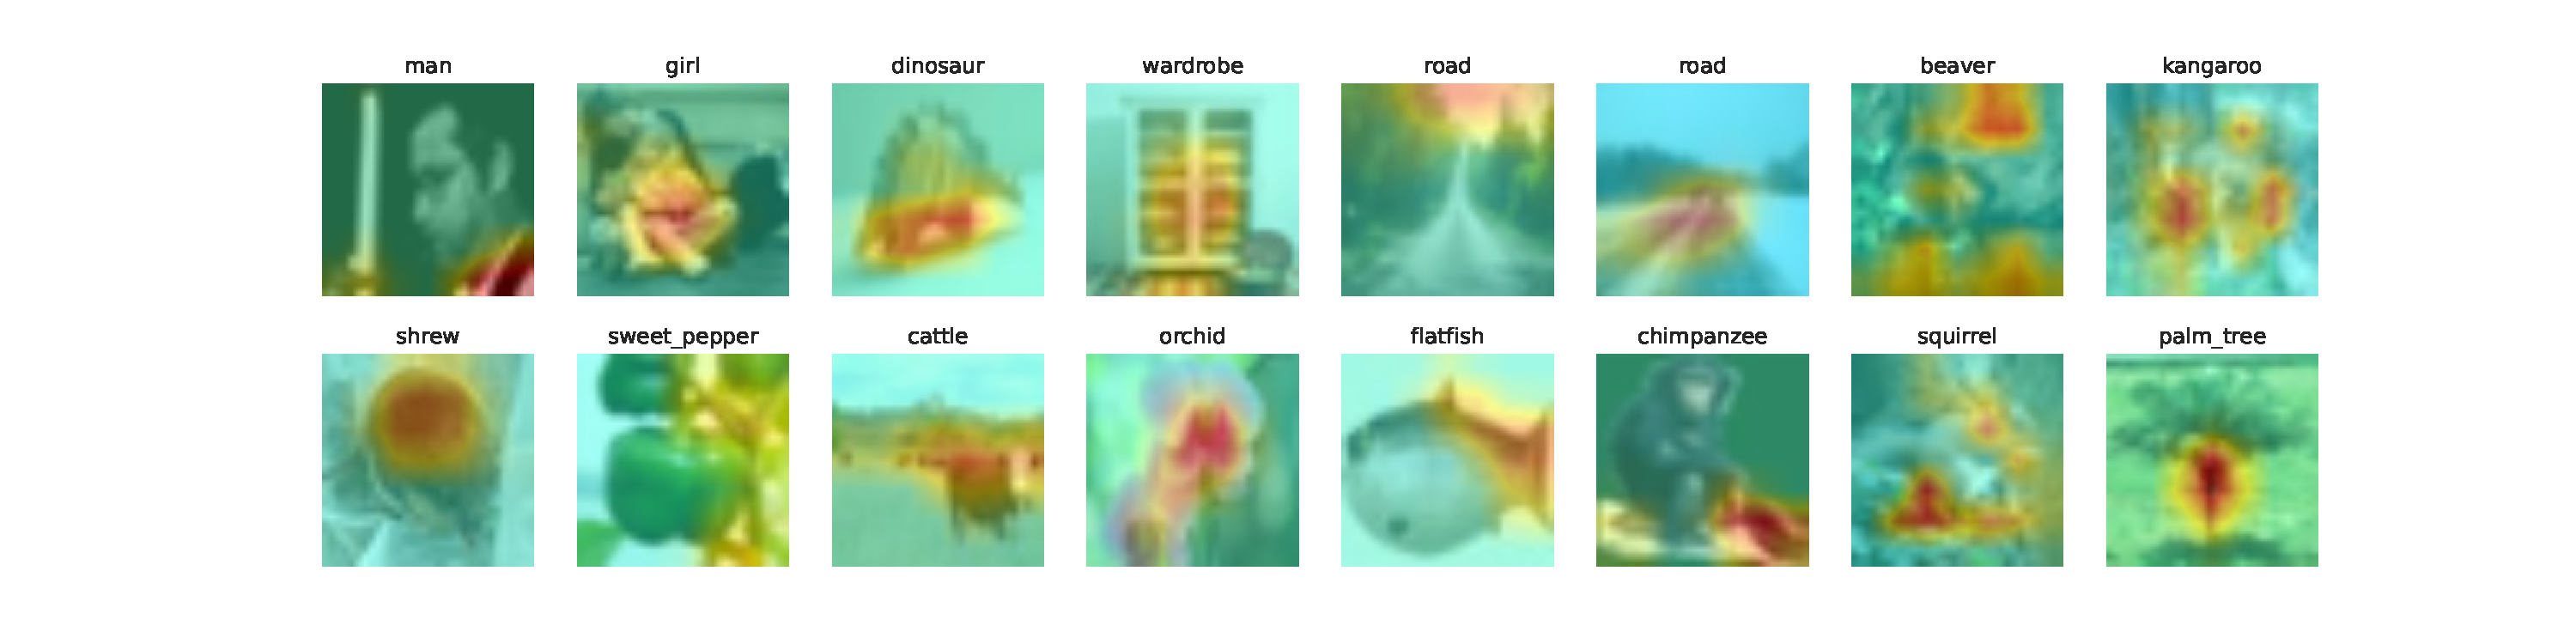
\includegraphics[width=\textwidth]{images/cifar100_efficientnet_b0_proxy_0.pdf}
            \caption{With Proxy Attention}
        \end{subfigure}
        \caption{Comparison of attention maps generated by efficientnet\_b0 trained with and without Proxy Attention on the cifar100 dataset}
    \end{figure}
    

    \begin{figure}[H]
        \centering
        \begin{subfigure}[b]{1\textwidth}
            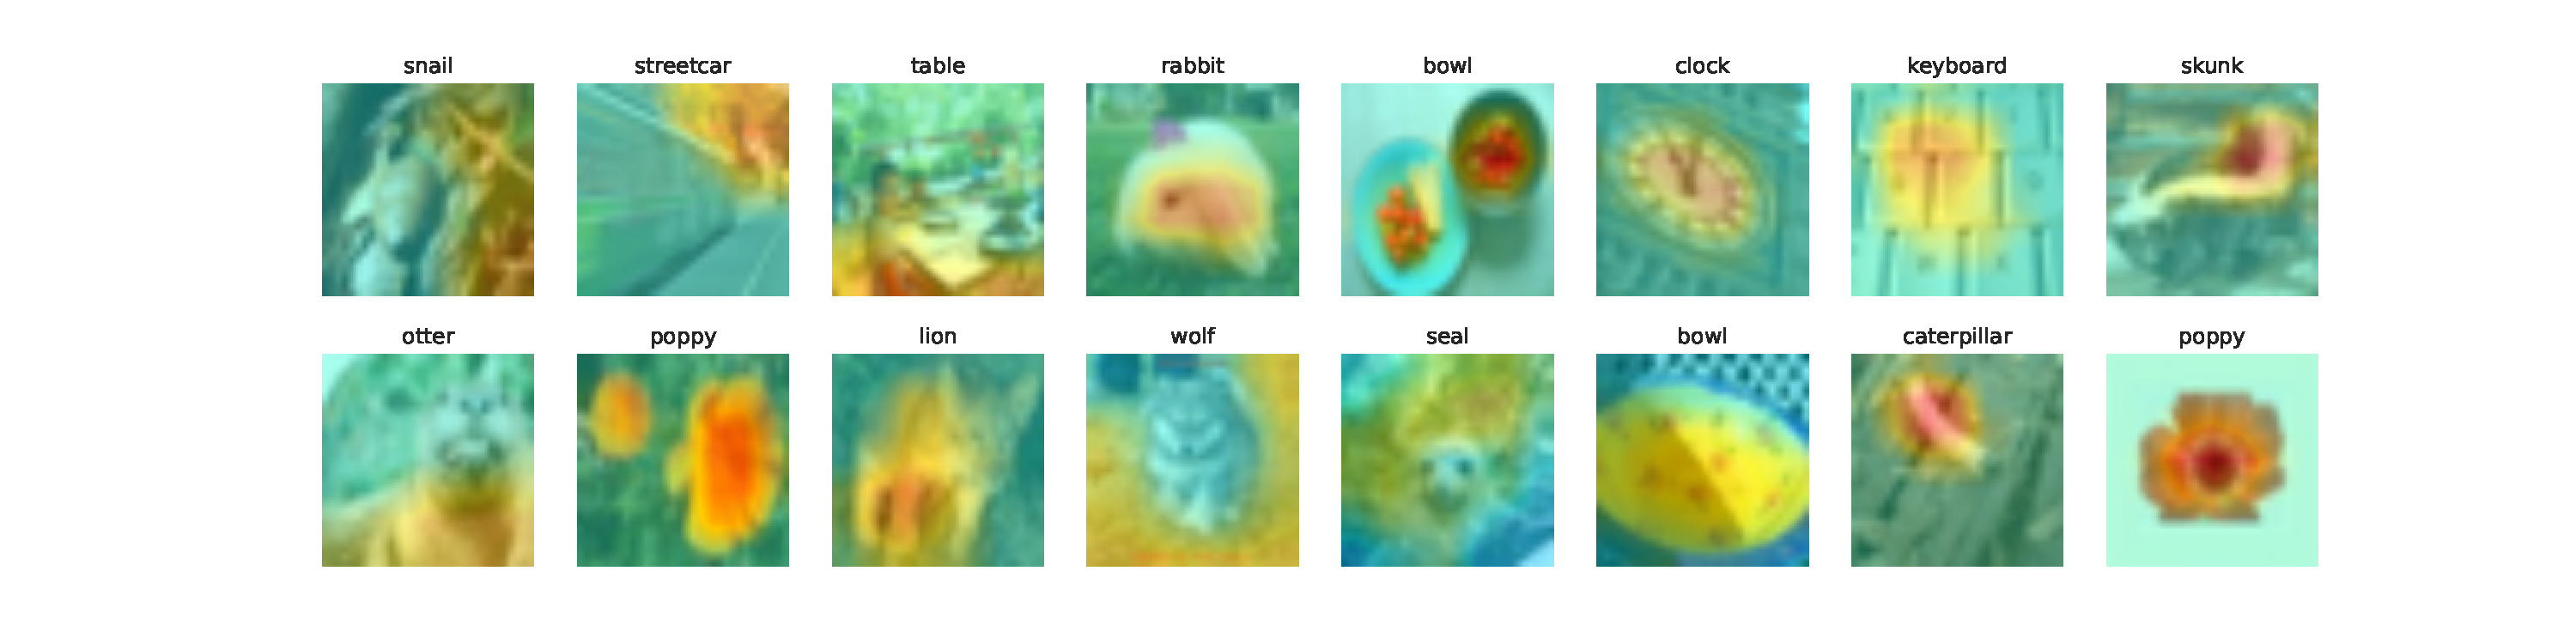
\includegraphics[width=\textwidth]{images/cifar100_efficientnet_b0_noproxy_0.pdf}
            \caption{Without Proxy Attention}
        \end{subfigure}
        \hfill
        \begin{subfigure}[b]{1\textwidth}
            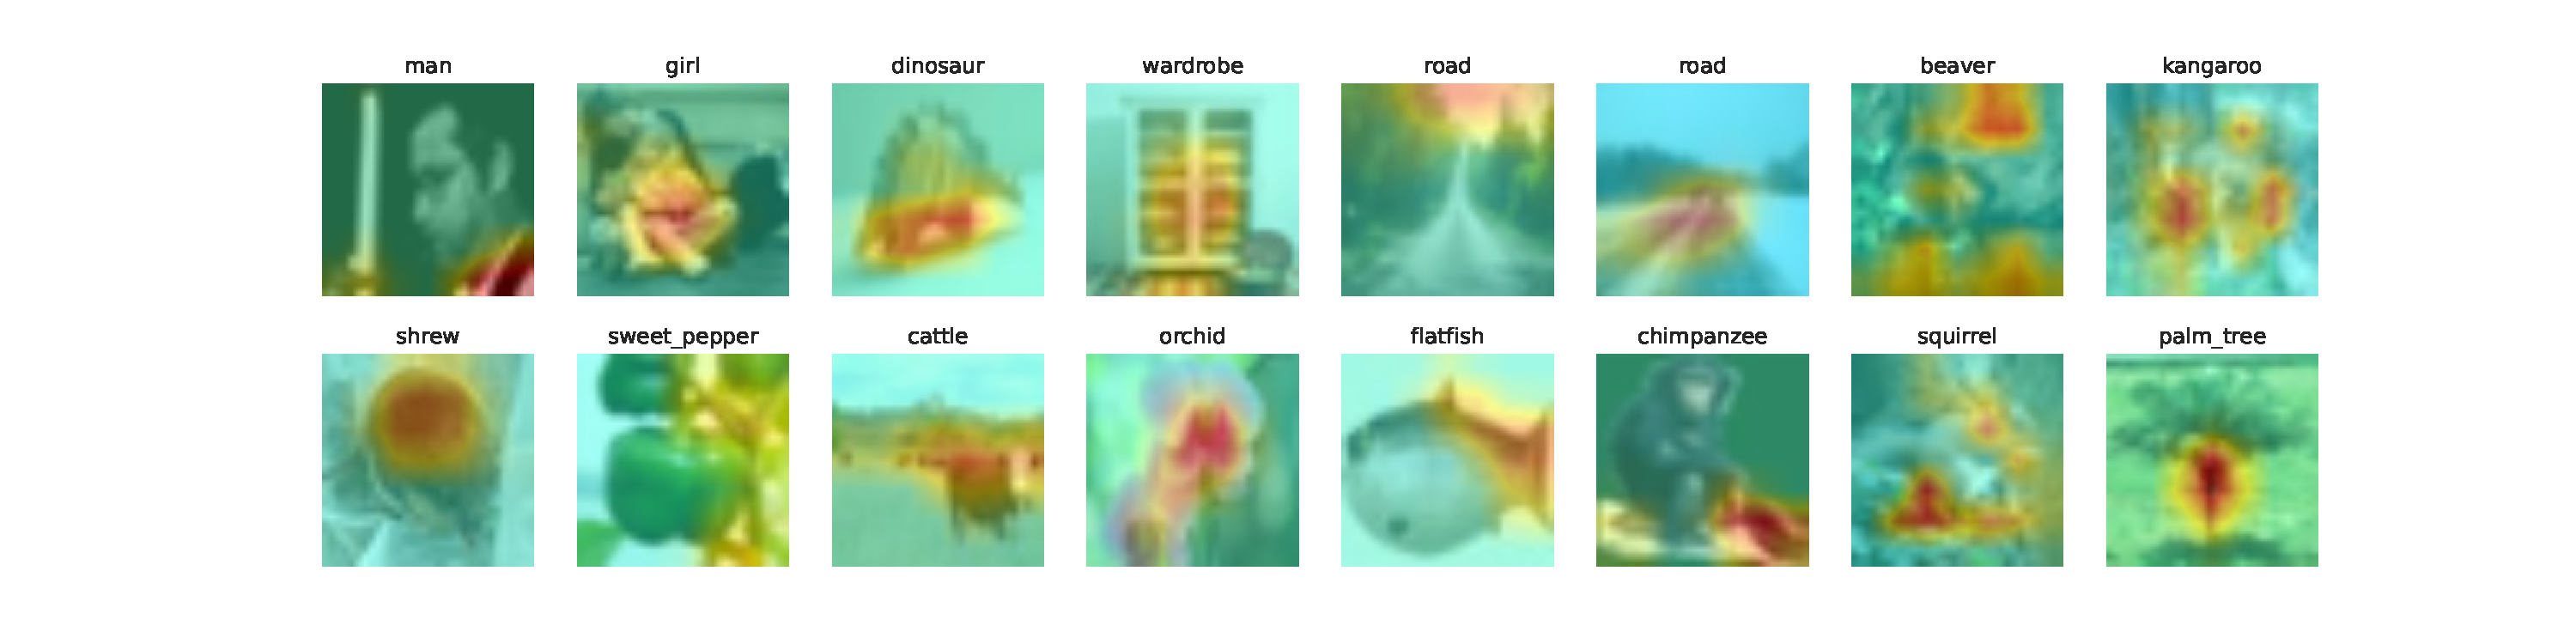
\includegraphics[width=\textwidth]{images/cifar100_efficientnet_b0_proxy_0.pdf}
            \caption{With Proxy Attention}
        \end{subfigure}
        \caption{Comparison of attention maps generated by efficientnet\_b0 trained with and without Proxy Attention on the cifar100 dataset}
    \end{figure}
    

    \begin{figure}[H]
        \centering
        \begin{subfigure}[b]{1\textwidth}
            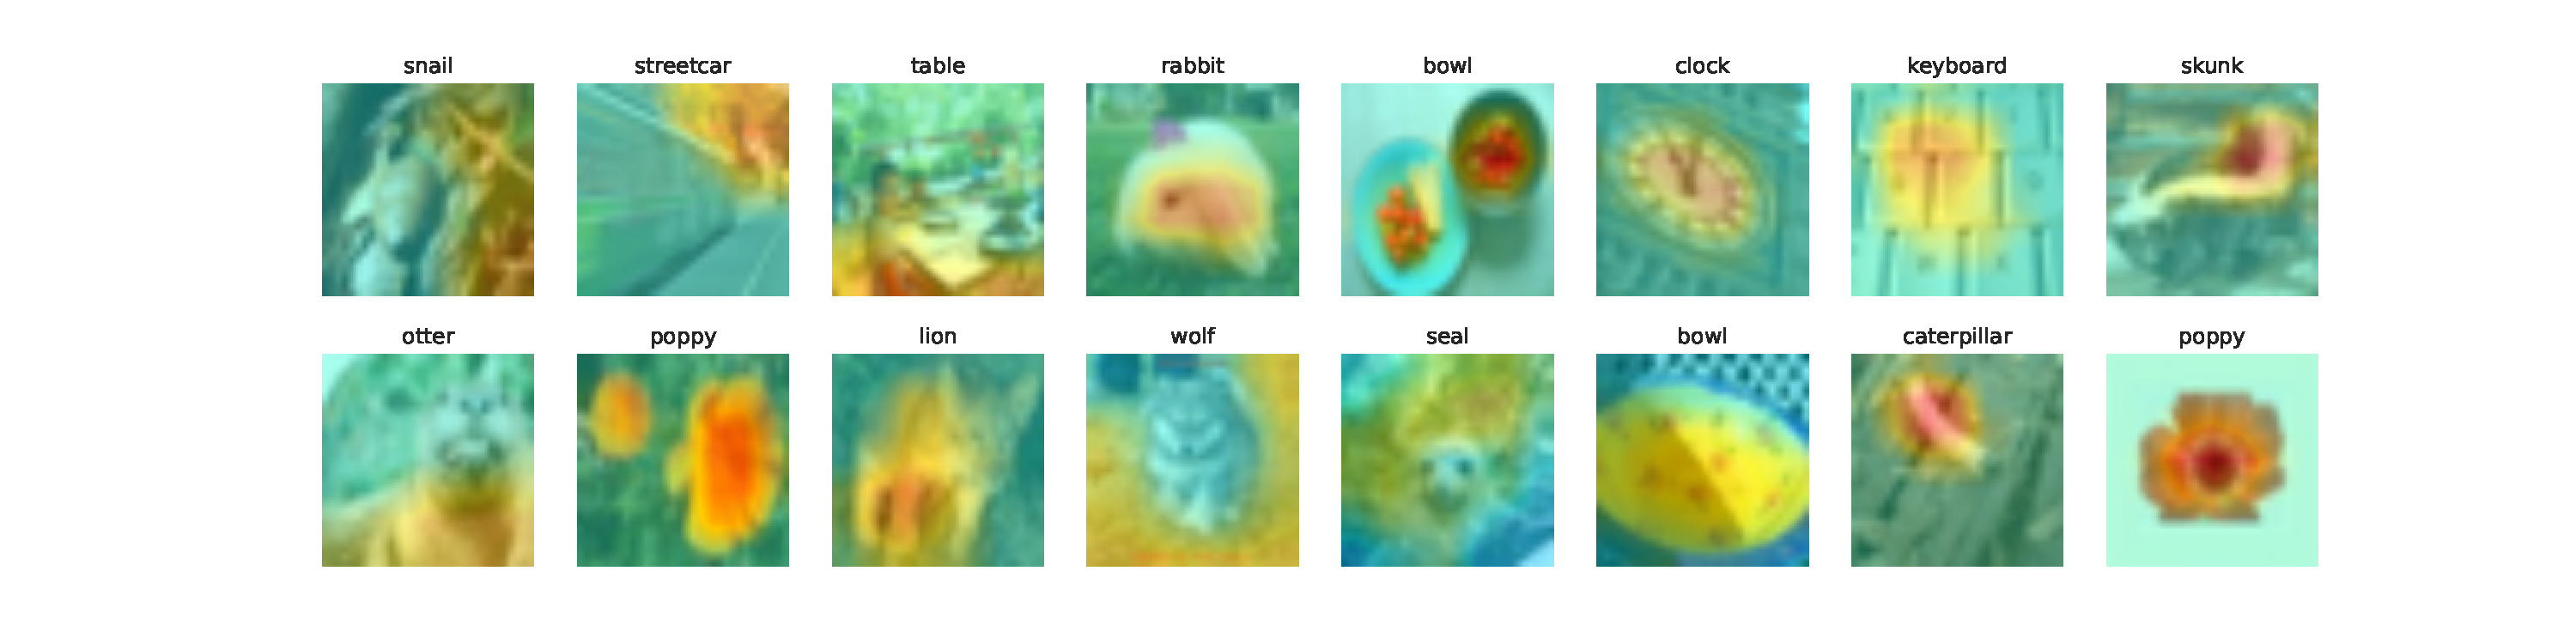
\includegraphics[width=\textwidth]{images/cifar100_efficientnet_b0_noproxy_0.pdf}
            \caption{Without Proxy Attention}
        \end{subfigure}
        \hfill
        \begin{subfigure}[b]{1\textwidth}
            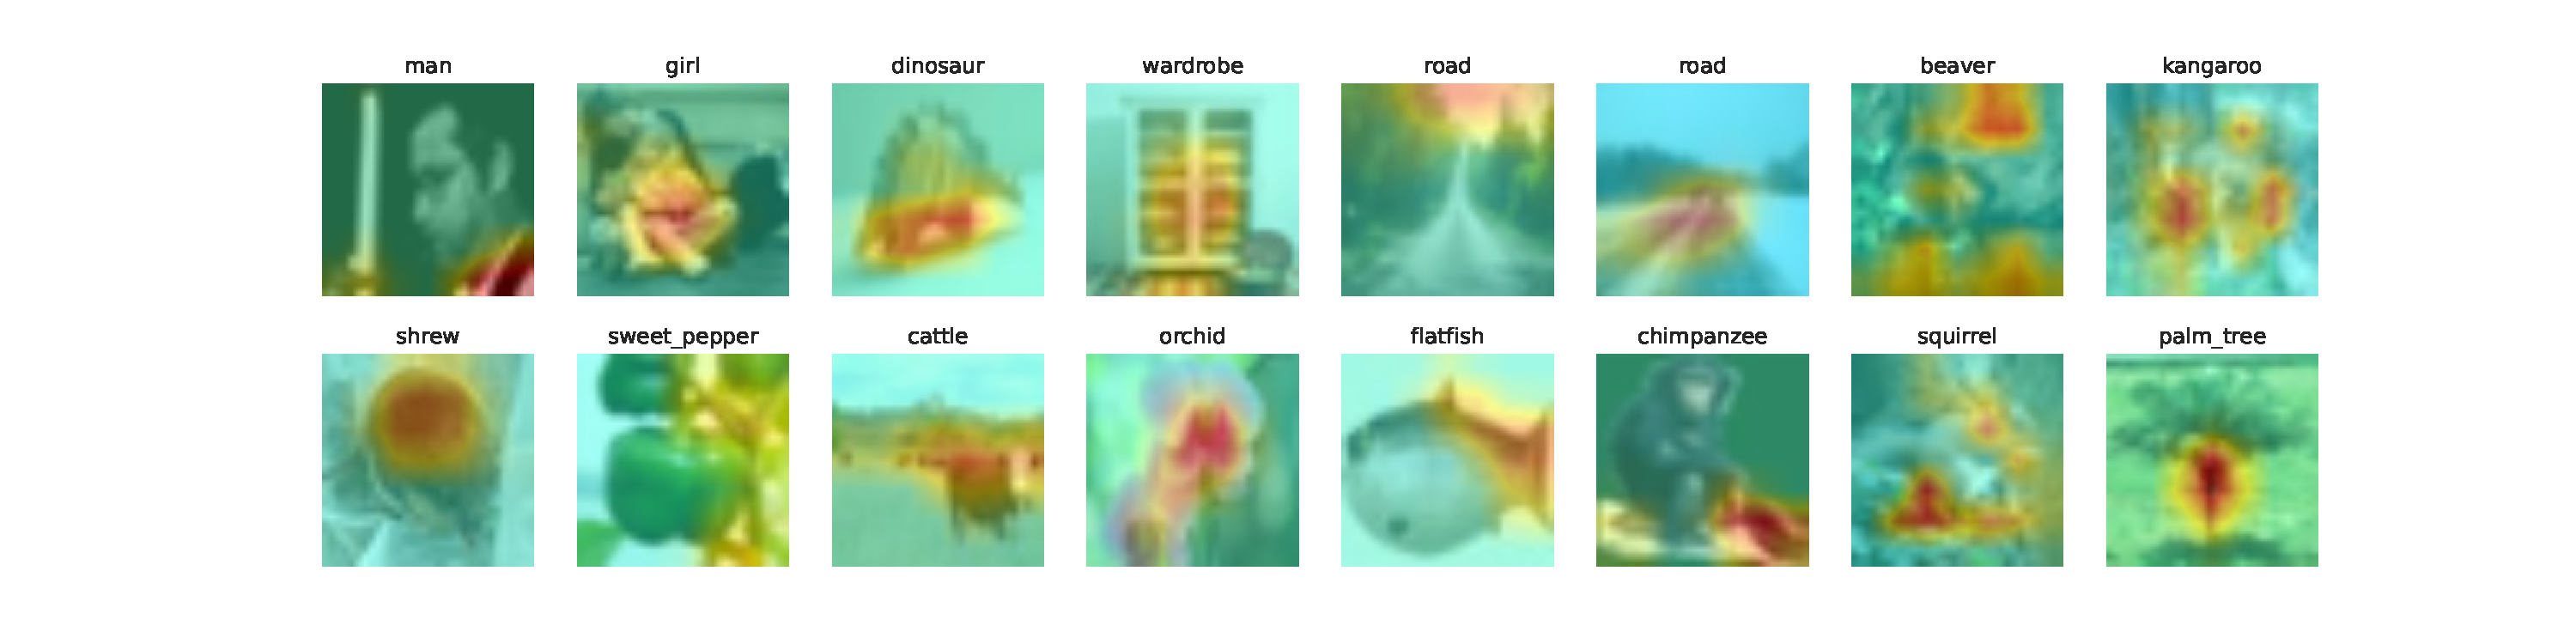
\includegraphics[width=\textwidth]{images/cifar100_efficientnet_b0_proxy_0.pdf}
            \caption{With Proxy Attention}
        \end{subfigure}
        \caption{Comparison of attention maps generated by efficientnet\_b0 trained with and without Proxy Attention on the cifar100 dataset}
    \end{figure}
    


\subsection{Tsinghua Dogs, ResNet18, EigenGradCAM}


% \thispagestyle{body}
\chapter{Conclusion} \label{ch:conclusion}

\section{Lessons Learned}
The lessons learned from this thesis are as follows:
\begin{itemize}
    \item \textbf{Combining research from different domains to create a novel method: } This thesis taught me how to combine research from different domains to create a novel method. In this case, we combined research from the domains of XAI and Augmentation to create a novel augmentation technique.
    \item \textbf{Hyperparameter Tuning: } We performed a large number of experiments with different hyperparameters and models to test the robustness of the method and find the best configuration. Doing so taught me the importance of hyperparameter tuning.
    \item \textbf{Memory Leaks: }We encountered a lot of memory leaks while working on the code for this thesis, and in the process learned how to debug and fix them. 
    \item \textbf{Function based code: }We wrote the code for this thesis in a functional style instead of an object oriented style as a personal experiment (inspired by the success of the Julia programming language). This made it easy to reuse certain parts of the code and modify others. Doing so taught me the importance of writing functional code.
    \item \textbf{Augmentation: }We learned a lot about augmentation while working on this thesis. We learned about the different types of augmentations, how to implement them, and how to use them to improve the performance of CNNs.
    \item \textbf{XAI: }We also learned a lot about XAI while working on this thesis. 
    \item \textbf{Training Loop: } Previous to this thesis, the author had only used the training loop provided by higher level libraries. However, for this thesis, we had to implement the training loop from scratch. Doing so taught the author a lot about the different components of the training loop and how to configure them for optimal performance and modify them to suit the needs of the project.
\end{itemize}

\section{Future Work}
While the results of this thesis are promising, there is still a lot of room for improvement. The following are some of the possible future directions for this work:
\begin{itemize}
    \item \textbf{Schedules:} Currently, the number of Proxy Steps and the number of images used for the Proxy Step are fixed. It would be interesting to schedule both of these based on the validation performance. For example, if the validation performance is not improving, we can increase the number of Proxy Steps and the number of images used for the Proxy Step.
    \item \textbf{More XAI methods:} We have only used a tiny subset of XAI methods for this thesis. It would be interesting to experiment with more XAI methods (eg: other methods from the literature survey) and see if they can be used to improve the performance of Proxy Attention.
    \item \textbf{Smoothing Attention Maps:} The attention maps generated by the XAI methods are noisy. While no extra smoothing was used in this thesis, it would be useful to experiment with smoothing the attention maps before using them for the Proxy step. An example of a potentially suitable smoothing method is Eigen Smoothing \cite{jacobPyTorchLibraryCAM2021}.
    \item \textbf{Better Attention Maps for ViT:} This research used the base vision transformer model but Abnar et al. \cite{abnarQuantifyingAttentionFlow2020} in their paper, find that the attention maps generated by a vision transformer are pretty unreliable due to self attention, combining different representations across layers of the transformer. While using self attention does lead to massive improvements and performance for Transformers, using these attention weights is an unreliable method of generating proper explanations. Thus future work could take their work into account to have a better comparison between CNNs and Transformers.
\end{itemize}

% \thispagestyle{body}
\chapter{Appendix}
\subsection{Summary of Results Per Dataset}
This section shows the accuracies per model for each dataset. The results are shown in Table ~\ref{tab:summary_ds}.
\begin{table}[H]
\centering
\resizebox{0.8\columnwidth}{!}{%
\begin{tabular}{lllr}
\toprule
         &                      &          &   accuracy \\
ds\_name & model & step\_schedule &            \\
\midrule
dogs & efficientnet\_b0 & Proxy &  94.630158 \\
         &                      & No Proxy &  85.605498 \\
cifar100 & vit\_base\_patch16\_224 & Proxy &  75.651538 \\
         &                      & No Proxy &  54.910000 \\
\bottomrule
\end{tabular}
}
\caption{Summary of results on different datasets}
\label{tab:summary_ds}
\end{table}
% \thispagestyle{body}

% \bibliographystyle{ieeetr}
% \bibliography{biblio}

% \chapter{Appendix}
\subsection{Summary of Results Per Dataset}
This section shows the accuracies per model for each dataset. The results are shown in Table ~\ref{tab:summary_ds}.
\begin{table}[H]
\centering
\resizebox{0.8\columnwidth}{!}{%
\begin{tabular}{lllr}
\toprule
         &                      &          &   accuracy \\
ds\_name & model & step\_schedule &            \\
\midrule
dogs & efficientnet\_b0 & Proxy &  94.630158 \\
         &                      & No Proxy &  85.605498 \\
cifar100 & vit\_base\_patch16\_224 & Proxy &  75.651538 \\
         &                      & No Proxy &  54.910000 \\
\bottomrule
\end{tabular}
}
\caption{Summary of results on different datasets}
\label{tab:summary_ds}
\end{table}
\printbibliography
\end{document}